\documentclass{article} % For LaTeX2e
\usepackage{iclr2027_conference,times}

% Optional math commands from https://github.com/goodfeli/dlbook_notation.
\input{math_commands.tex}

\usepackage{hyperref}
\usepackage{url}
\usepackage{amsmath}
\usepackage{amssymb}
\usepackage{booktabs}
\usepackage{graphicx}
\usepackage[section]{placeins}
\usepackage{amsthm}
\usepackage{xcolor}
\usepackage[framemethod=default]{mdframed}
% Formal statements stand apart from the running argument, with a light tint and a
% colored rule, allowing a reader to find them by scanning. Definitions carry a warm
% amber tint with an amber heading, propositions a neutral grey.
\definecolor{defbg}{RGB}{255,251,235}
\definecolor{defrule}{RGB}{214,168,46}
\definecolor{defhead}{RGB}{140,98,10}
\newtheoremstyle{defstyle}% name
  {0pt}{0pt}%                    space above and below, handled by the frame
  {\normalfont}%                 body font
  {}%                            indent
  {\bfseries\color{defhead}}%    head font
  {.}%                           punctuation after head
  {0.5em}%                       space after head
  {}%                            head spec
\mdfdefinestyle{defbox}{%
  backgroundcolor=defbg, linecolor=defrule, linewidth=0.7pt,
  innertopmargin=7pt, innerbottommargin=7pt,
  innerleftmargin=10pt, innerrightmargin=10pt,
  skipabove=8pt, skipbelow=8pt, roundcorner=3pt,
  % a boxed statement split over a page break loses its bottom rule and strands
  % the display equation, therefore the whole box moves together
  nobreak=true}
\mdfdefinestyle{thmbox}{%
  backgroundcolor=black!4, linecolor=black!30, linewidth=0.4pt,
  innertopmargin=4pt, innerbottommargin=4pt,
  innerleftmargin=7pt, innerrightmargin=7pt,
  skipabove=6pt, skipbelow=6pt, roundcorner=1pt,
  nobreak=true}
\theoremstyle{defstyle}
\newmdtheoremenv[style=defbox]{definition}{Definition}
\theoremstyle{plain}
\newmdtheoremenv[style=thmbox]{proposition}{Proposition}
\usepackage{wrapfig}
\usepackage{enumitem}
\usepackage{needspace}


\title{Less Than Meets the Eye: \\Action-Set Identifiability and Principled\\Abstention for 3D Physical Geometry}

% Authors must not appear in the submitted version. They should be hidden
% as long as the \iclrfinalcopy macro remains commented out below.
% Non-anonymous submissions will be rejected without review.
\author{Anonymous authors \\ Paper under double-blind review}

\newcommand{\fix}{\marginpar{FIX}}
\newcommand{\new}{\marginpar{NEW}}

% The paper is float-heavy and the LaTeX defaults leave wide bands of white
% above and below every float; these lengths tighten that without touching
% the ICLR type area.
\setlength{\floatsep}{6pt plus 2pt minus 2pt}
\setlength{\textfloatsep}{8pt plus 2pt minus 2pt}
\setlength{\intextsep}{7pt plus 2pt minus 2pt}
\setlength{\abovecaptionskip}{4pt}
\setlength{\belowcaptionskip}{2pt}
\setlength{\abovedisplayskip}{4pt plus 1pt minus 2pt}
\setlength{\belowdisplayskip}{4pt plus 1pt minus 2pt}
\setlength{\abovedisplayshortskip}{3pt}
\setlength{\belowdisplayshortskip}{3pt}
\renewcommand{\arraystretch}{1.02}
% The results section is float-dense. These fractions let a page carry more float
% material before LaTeX defers a float to a page of its own, which is what strands
% figures among blank space, while \textfraction keeps some text on every page.
\renewcommand{\topfraction}{0.9}
\renewcommand{\bottomfraction}{0.6}
\renewcommand{\textfraction}{0.12}
\renewcommand{\floatpagefraction}{0.75}

%\iclrfinalcopy % Uncomment for camera-ready version, but NOT for submission.
\begin{document}

\maketitle
% The title block and abstract fill page 1; suppress top floats there so the
% teaser cannot be hoisted above the title.
\suppressfloats[t]

\begin{abstract}
A depth prediction can match its reference measurement and still describe a surface that no
hand would touch. A corridor, the reflection of that corridor in a planar mirror, and a
photograph of the corridor on a screen can produce one image, while a hand stops in three
different places. Existing work meets such scenes by enlarging what a predictor
represents or reports, through multi-layer formulations that retain a transparent interface
together with the scene behind that interface, through detectors for mirrors and glass, and
through uncertainty estimation and conformal prediction that attach a calibrated scalar to
each answer. Each such quantity describes a prediction or a predictor at a fixed viewpoint,
and none registers that the observation itself carries no evidence, because one image stays
consistent with every explanation. We therefore ask a
different question. Given the camera motions available to an observer, can the physical
explanation be recovered at all? Two explanations become separable to the extent that
they predict different observations after the camera moves. A scene counts as identifiable
when at least one available motion separates every remaining explanation, and the system
abstains otherwise, while a maximin rule selects the motion separating the weakest
contending pair. On a benchmark whose competing explanations are pixel-identical at the
reference view, abstention lowers false physical certainty from $0.832$ to $0.000$, and
maximin selection reaches a committed accuracy of $1.000$ across four mechanisms, against
$0.587$ on mirrors for a belief-weighted objective. On real photographs, all thirteen
checkpoints from seven architecture families fail on $59.5$ to $78.4\%$ of images, while
their own confidence stays below chance at predicting these failures. Choosing the viewpoint
that some hypothesis explains best lowers ambiguous-region error by $31.3\%$ on all thirteen
checkpoints, and a gate over frozen encoder features reaches $0.887$ out of fold and lowers
the failure rate from $65.2\%$ to $50.2\%$ at $70\%$ coverage.
\end{abstract}

%============================================================================
% INTRODUCTION
%============================================================================
\section{Introduction}
\label{sec:introduction}

A corridor viewed through an open doorway, the same corridor reflected in a planar mirror,
and a photograph of that corridor on a screen can produce an identical image. The three
scenes differ in the surface a hand would touch, namely empty air, a pane of glass, and a
rigid panel, while the light reaching the sensor stays the same. An image therefore
does not determine the physical explanation of the observed geometry, and an answer produced
from that image alone follows a prior rather than evidence. One change of viewpoint, by contrast,
separates the three arrangements at once, because a doorway, a pane of glass, and a rigid
panel send light along different paths as soon as the camera moves. Wherever perception drives
action, as when a service robot separates a doorway from a reflection before committing to a
path, physical contact sets the cost of such an error, and the quantity of interest becomes
the geometry of the first real surface along the ray. Figure~\ref{fig:system} follows one
real photograph through the decision proposed here, up to the point at which the available
evidence cannot choose between the competing explanations.

\begin{figure}[!t]
\begin{center}
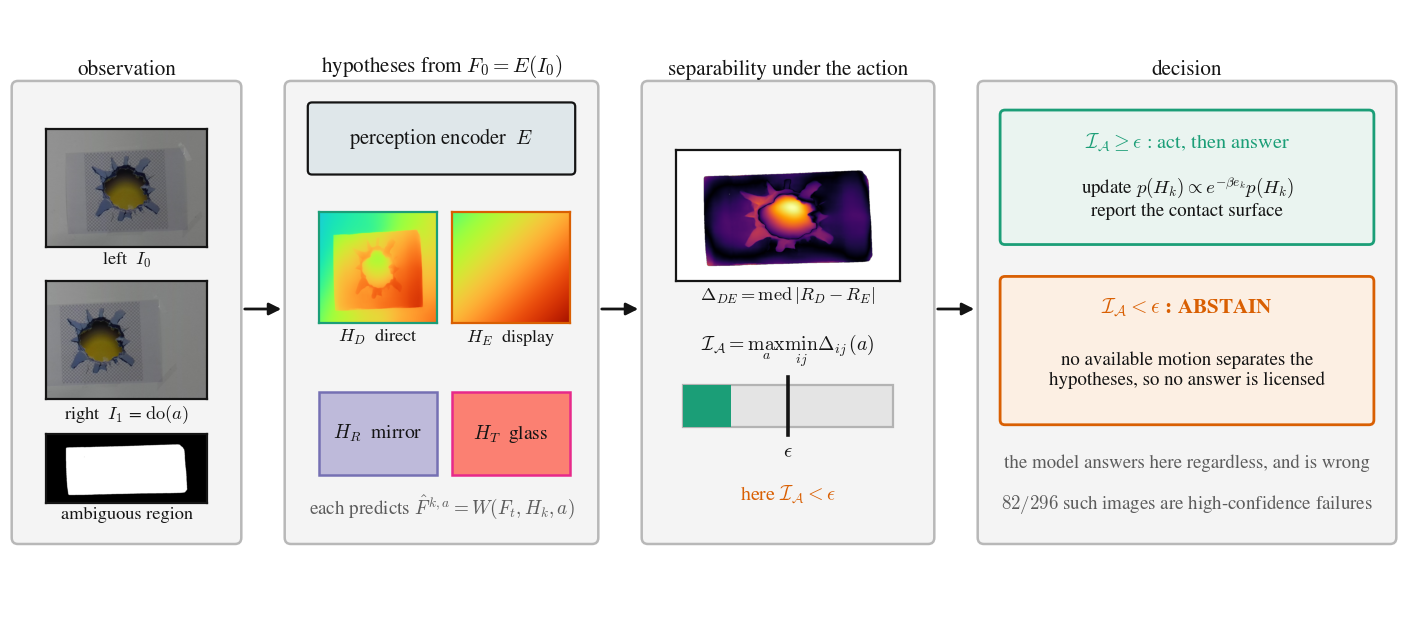
\includegraphics[width=0.73\linewidth]{figures/fig_system.png}
\end{center}
\caption{\textbf{The method, followed through one real image.} A stereo pair provides the executed action
and the annotated region marks where the surface becomes ambiguous. The encoder geometry
yields $H_D$ and, after a plane fit over that region, $H_E$. Warping the second view under
each hypothesis produces the separability $\Delta_{DE}$ of \eqref{eq:delta-photometric},
whose identifiability falls below the perceptual threshold, and \eqref{eq:abstain} therefore
declines to answer on a scene that the predictor answers wrongly.}
\label{fig:system}
\end{figure}

Several lines of work already extend perception toward such configurations, through
multi-layer formulations that retain both a transparent interface and the scene behind that
interface \citep{layereddepth2025,seegroup2026,depthfocus2026}, through detectors for
mirrors and glass \citep{mirror3d2021,glint2026}, and through selective prediction
\citep{chow1970} with split conformal prediction \citep{vovk2005,lei2018} that decides when
a system should answer. Together these lines address what the depth is, which surfaces are
present, where the camera should move next, and how certain a prediction is, and the matched
configurations above therefore raise a prior question. Can an observer recover the physical
explanation at all from the available observations?

The question stands apart from accuracy and from uncertainty. Accuracy describes a
prediction and uncertainty describes a predictor, whereas identifiability describes the
triple formed by the competing explanations, the actions available to the observer, and the
resolution at which differences become perceptible. For a view-tracked display observed
within its aperture, the answer is not merely difficult to obtain, because the available
evidence does not contain that answer. Enlarging a model or gathering further images from
the same viewpoint therefore changes nothing, whereas a suitable change of viewpoint
resolves the case at once. We accordingly define identifiability relative to an action set,
and we treat the label \emph{not identifiable} as a statement about that triple. The framing
holds independently of architecture, because a scalar confidence carries no mechanism for
registering absent evidence where one image stays consistent with every hypothesis.

\paragraph{Contributions.}

\begin{enumerate}[nosep,leftmargin=*,topsep=2pt]

\item \textbf{Action-set identifiability and intervention selection.} We define separability
under camera motion, identify a scene only when some available action separates every
remaining hypothesis beyond a perceptual threshold, and select actions by maximin
separability, a criterion that optimal design knows as $T$-optimality
\citep{atkinson1975design,hunter1965experimental}.

\item \textbf{A benchmark and protocol with measured ambiguity.} Our cases remain
pixel-identical at the reference view to order $10^{-14}$~px and include instances that no
action resolves, which makes correct abstention measurable, while calibrated stereo provides
the executed action on real images.

\item \textbf{Evidence that the failure spans architectures and scenes.} Thirteen
checkpoints from seven architecture families report depicted rather than physical geometry on
$59.5$ to $78.4\%$ of images, and on $67.0\%$ of $123$ photographs of real mirrors, while
their confidence stays below chance at predicting these errors.

\item \textbf{A predictor-agnostic abstention gate.} A head over frozen encoder features
predicts failures at $0.887$ out of fold, transfers across all $13$ held-out checkpoints,
and lowers the failure rate from $65.2\%$ to $50.2\%$ at $70\%$ coverage.

\end{enumerate}


%============================================================================
% METHOD
%============================================================================
\section{Method}
\label{sec:method}

The method maintains a set of competing physical explanations for an observed image,
predicts what each explanation implies for every candidate camera motion, and answers only
when some available motion separates every explanation still in contention.
Table~\ref{tab:supp-notation} collects the notation and Figure~\ref{fig:pipeline} presents
the pipeline.

\subsection{Hypotheses and the Action Set}
\label{sec:formulation}

Let $I_0$ denote an image at reference pose $C_0$, and let $F_0 = E(I_0)$ denote the
geometry that a perception encoder $E$ reports for that image, expressed as landmarks
carrying image coordinates, depths, and visibility flags. \begin{definition}[Image-formation hypothesis family]\label{def:hypotheses}
Rather than $F_0$ alone, the method keeps a four-member family
$\mathcal{H} = \{H_D, H_E, H_R, H_T\}$. The observed structure is physically present,
depicted on a flat emissive panel, the virtual image of a real scene in a planar
mirror, or seen through a plane-parallel transparent slab. Each hypothesis places the
first touchable surface elsewhere, and all four remain \emph{matched} at $C_0$, being
pixel-identical there, and any separation gained after a motion therefore follows from
the motion alone.
\end{definition} Against that family the observer acts. An action $a \in SE(3)$ applies a
rigid camera motion as an explicit intervention $\mathrm{do}(C_1 = C_0 \cdot a)$, where the
do-operator replaces conditioning because the observer chooses the viewpoint. Actions come
from a bounded set $\mathcal{A}$ of translations of $\{0.05, 0.10, 0.20, 0.30\}$~m along
three axes, rotations of $\{5^\circ, 10^\circ\}$ in yaw and pitch in both directions, and
the null action, which yields $|\mathcal{A}| = 33$ within the $0.35$~m and $15^\circ$ budget
of a small corrective movement. A finite action set allows evaluation of identifiability by
enumeration before any motion, and abstention therefore becomes possible before acting.

\subsection{Predicting the Consequence of an Action}
\label{sec:transition}

Each hypothesis maps current geometry and a candidate action to a predicted observation,
\begin{equation}
\label{eq:transition}
\hat{F}^{\,k,a} \;=\; W\!\left(F_t,\, H_k,\, a\right),
\end{equation}
where $F_t$ denotes the geometry at time $t$, $H_k$ the $k$-th hypothesis, and
$\hat{F}^{\,k,a}$ what $H_k$ predicts after execution of $a$. The transition $W$ applies
one shared projection to every hypothesis and differs only in the world that each
hypothesis asserts, and any difference between predictions therefore follows from the
mechanism alone. The mechanisms remain planar because planarity keeps every transition
closed form. Display content maps between views by the plane-induced homography
$K'(R - t\mathbf{n}^{\top}/d)K^{-1}$, a planar mirror reflects exactly across its plane,
where the camera pose transforms by the Householder map
$\mathbf{R} \mapsto (I - 2\mathbf{n}\mathbf{n}^{\top})\mathbf{R}$ with translation
$-2d\mathbf{n}$, and a planar slab displaces content axially by $d\,(1 - 1/n)$. Closed form
in turn makes the counterfactuals \emph{matched}, because reference views then coincide to
numerical precision and divergence after an action cannot arise from approximation error. A
curved surface admits no exact transition, and a learned transition would reintroduce the
confound that the shared projection removes, although the formalism remains independent of
that restriction (Appendix~\ref{sec:supp-extension}).

\subsection{Separability, Identifiability, and Abstention}
\label{sec:separability}

Pairwise separability measures the distance between the consequences that two hypotheses
predict for the same action, where $i,j$ index two hypotheses and $D$ denotes a composite
distance,
\begin{align}
\label{eq:separability}
\Delta_{ij}(a) \;&=\; D\!\left(\hat{F}^{\,i,a},\, \hat{F}^{\,j,a}\right), \\
\label{eq:distance}
D \;&=\; \lambda_m D_{\text{motion}} + \lambda_o D_{\text{occlusion}}
      + \lambda_g D_{\text{geometry}} + \lambda_f D_{\text{feature}} .
\end{align}
The motion term measures the root-mean-square image-space displacement between the two
predicted landmark sets over jointly visible landmarks, in pixels, and the occlusion term
counts landmarks whose predicted visibility differs, with visibility decided by z-buffering
the geometry of each hypothesis. The geometry term measures the root-mean-square
three-dimensional distance between back-projected landmarks, and the feature term measures a
learned appearance distance that remains unused here. Throughout the experiments
$\lambda_m = 1$, $\lambda_o = 4.0$~px, and $\lambda_g = \lambda_f = 0$, which places $D$ in
pixels and raises one unambiguous appearance or disappearance, often the only cue a mirror
offers, clearly above the threshold introduced below (Appendix~\ref{sec:supp-occlusion}).
The quantity of interest then becomes the best separability that the action set attains, and
a pair counts as separable when any permitted motion distinguishes that pair. The system
abstains when no permitted motion does,
\begin{align}
\label{eq:identifiability}
\mathcal{I}_{\mathcal{A}}\!\left(H_i, H_j\right)
\;&=\; \max_{a \in \mathcal{A}} \; \Delta_{ij}(a), \\
\label{eq:abstain}
\min_{(i,j)} \; \mathcal{I}_{\mathcal{A}}\!\left(H_i, H_j\right) \;&<\; \epsilon ,
\end{align}
with the minimum running over pairs still in contention. The order of the two operators
matters. A maximum over actions inside a minimum over pairs licenses an answer only when
some action separates every undecided pair, and the pair left unseparated marks exactly
where an error would occur. Priors over hypotheses remain uniform at $t = 0$, and the
threshold $\epsilon = 1.0$~px follows from the sensor and the perceptual criterion rather
than from tuning, with Appendix~\ref{sec:supp-sensitivity} sweeping that threshold.

\subsection{Choosing the Intervention}
\label{sec:selection}

We compare two objectives. The first objective sums separabilities, as active perception
commonly does,
\begin{equation}
\label{eq:sum}
a^{\star}_{\text{sum}} \;=\; \arg\max_{a \in \mathcal{A}}
\;\sum_{i<j} p_i\, p_j\, \Delta_{ij}(a),
\end{equation}
where the posteriors $p_i, p_j$ let still-plausible pairs contribute more. Such a sum,
however, can reach its maximum at an action that separates pairs outside contention while
leaving the deciding pair unseparated, and the second objective therefore replaces the sum
with the weakest contending pair,
\begin{equation}
\label{eq:maximin}
a^{\star}_{\text{maximin}} \;=\; \arg\max_{a \in \mathcal{A}}
\;\min_{(i,j) \in \mathcal{C}} \; w_{ij}\, \Delta_{ij}(a),
\end{equation}
where $\mathcal{C}$ collects pairs whose joint posterior mass has not collapsed and
$w_{ij}$ weights each pair by that mass. The form follows from the abstention rule, because
a decision requires every contending pair separated and the binding quantity therefore
becomes the smallest separability. Optimal design for model discrimination knows this
criterion as $T$-optimality \citep{atkinson1975design,hunter1965experimental}, and the
present work transfers the criterion to active vision. The two objectives differ only where
at least two hypothesis pairs exist, as in the six pairs of the synthetic benchmark and not
in a stereo pair, and selection on real photographs therefore runs through the belief update
of \eqref{eq:belief}. Among viewpoints that the observer could occupy, the rule prefers the
one at which some hypothesis best accounts for the view obtained,
\begin{equation}
\label{eq:evidence-selection}
a^{\star}_{\text{evidence}} \;=\; \arg\min_{a \in \mathcal{A}} \;
\min_{k} \; e_k(a),
\end{equation}
with $e_k(a)$ the residual of hypothesis $k$ after execution of $a$. Both rules act on the
same machinery, one through the separability entering the belief and the other through the
residual leaving that belief.

\subsection{Belief Update and Output}
\label{sec:belief}

After execution of the selected action and observation of $O'$, each hypothesis carries the
residual $e_k = D(\hat{F}^{\,k,a^\star}, E(O'))$ under the same
distance~\eqref{eq:distance}, and prediction error therefore shares a scale with
separability. The belief updates multiplicatively,
\begin{equation}
\label{eq:belief}
p_{t+1}(H_k) \;\propto\; \exp\!\left(-\beta\, e_k\right)\, p_t(H_k),
\end{equation}
where $\beta$ converts pixel error into log-likelihood and $\beta = 1.0$ makes a one-pixel
error cost one nat, while a posterior floor stops one unlucky observation from eliminating
a hypothesis permanently. The system then names the mechanism and reports the contact
geometry, the first physical surface along each ray, the glass for a mirror and the panel
for a display. The system withholds commitment when the posterior maximum does not exceed
$\tau = 0.45$, a value just below the $0.5$ tie that a forced choice over a two-way
ambiguity produces.

\subsection{Protocol for Real Photographs}
\label{sec:real-protocol}

Real data requires no change to the method, because a calibrated rectified stereo pair
already constitutes an executed action with known parameters and real photographs therefore
have $|\mathcal{A}| = 1$. The setting demands only that no step absorb the effect under
measurement. A monocular predictor returns relative inverse depth, defined up to an unknown
scale and shift, and we fit both quantities by least squares against reference disparity
outside the ambiguous region and apply them inside that region, which yields the disparity
predicted under $H_D$,
\begin{equation}
\label{eq:align}
d_{D} \;=\; s\,\hat{p} + t ,
\end{equation}
where $\hat{p}$ denotes the raw prediction, $s$ the scale, and $t$ the shift. Fitting
\eqref{eq:align} where the predictor performs well, and scoring where the predictor
performs poorly, stops those two parameters from absorbing the discrepancy under study. The
competing flat-panel hypothesis is the least-squares plane through that aligned prediction,
fitted to the prediction and not to the reference, because a hypothesis built from the
answer would place ground truth inside a test-time quantity. We then evaluate separability
in the image. Rectification aligns the pair, therefore column $x$ with disparity $d$
corresponds to column $x - d$ in the other view, and the right photograph warps into the
left frame under each hypothesis before we compare the two warps,
\begin{align}
\label{eq:warp}
R_{k}(x, y) \;&=\; I_{\text{right}}\!\left(x - d_{k}(x,y),\; y\right),
\qquad k \in \{D, E\}, \\
\label{eq:delta-photometric}
\Delta_{DE} \;&=\; \operatorname{median}\left|R_{D} - R_{E}\right| ,
\end{align}
with $d_k$ the disparity that hypothesis $k$ predicts and the median taken over pixels where
both warps remain valid. Warping the same photograph twice cancels illumination, sensor
noise, and rectification error, and the result carries intensity units, therefore a
disagreement counts only where the image carries structure to reveal that disagreement. A
featureless region, where the hypotheses predict different geometry and identical pixels,
then enters the record as unidentifiable at any baseline, whereas a disparity-space measure
would call the same region highly identifiable. Two commitments remain. A physical sheet or
panel is flat, and we therefore retain an image only when a plane fitted to the reference
disparity inside the region attains $R^2 \geq 0.90$, below which the stereo reference has
locked onto displayed content rather than onto the panel. Failure follows a definition
independent of every signal under test, since a predictor fails when its relative error
inside the region exceeds its error outside that region, a label that mentions neither
confidence nor identifiability. Every value of the area under the receiver operating
characteristic curve (AUROC) follows the convention that a larger value indicates a more
likely error.

%============================================================================
% RESULTS
%============================================================================
\section{Results}
\label{sec:results}

\subsection{Experimental Setup}
\label{sec:setup}

The synthetic benchmark instantiates each base scene under every mechanism and adjusts
content until the reference views coincide to order $10^{-14}$~px, which makes chance-level
single-view performance a verified property of the data and attributes any later gain to the
executed action. The benchmark also retains configurations that no permitted action
resolves, because a benchmark of only resolvable cases would score a method that answers
everywhere as highly as one that abstains where abstention is warranted, and splits follow
base scenes, which stops a memorized scene identity from standing in for a recovered
mechanism. We report causal explanation accuracy (CEA), which counts abstention as an error,
committed accuracy, which measures what an answer is worth once given, the false physical
certainty rate (FPCR), which counts confident commitments on unresolvable cases, and
normalized regret against the best available action, all defined in
Table~\ref{tab:supp-metrics}.

Every model evaluated here remains frozen and we fit only a small policy on top, which turns
the learned component into a question about read-out, namely whether the quantities a
network already computes suffice to predict its own failures. One policy takes the
hand-designed quantities of Section~\ref{sec:method} as input, and the other takes the
frozen intermediate features of the network, pooled over the ambiguous region as contrasts
against the surroundings of that region. We split folds by base scene, choose
hyperparameters on inner folds, score only on outer folds, and train under a
leave-one-model-out protocol that asks whether failure describes the image rather than one
network (Appendix~\ref{sec:supp-learned}). We use thirteen checkpoints as released, spanning
seven architecture families and a $38\times$ range in parameter count, with no training or
tuning on any evaluation set.

\subsection{Synthetic Benchmark}
\label{sec:res-synth}

Table~\ref{tab:phase1} reports Phase~1 over $11$ seeds with the benchmark redrawn per seed,
and the intervals therefore reflect the data-generating process. The single-view classifier
stays at exactly chance in every seed, which confirms that the matched construction leaves
nothing for one view to exploit, and the ordering from single-view to passive to
intervention-aware holds strictly in $11$ of $11$ seeds. A second study then isolates the
choice of intervention. The summed objective \eqref{eq:sum} reaches $0.587$ and $0.956$
committed accuracy on mirrors, where maximin selection \eqref{eq:maximin} reaches $1.000$
in each case (Figure~\ref{fig:main}c), and across four mechanisms maximin selection exceeds
the passive baseline by $+0.297$ ($t = 41.6$, $11$ of $11$ seeds). A belief-weighted sum can
reach its maximum at an action that separates pairs outside contention while leaving the
deciding pair unseparated, and the gap therefore has a structural origin, because an action
scoring zero on a pair cannot separate that pair at any $\epsilon$.

\begin{table}[t]
\caption{\textbf{Choosing the intervention decides the outcome on the synthetic benchmark.} Eleven
seeds per method, where chance stands at $0.333$ and CEA counts abstention as an error.}
\label{tab:phase1}
\begin{center}
\footnotesize
\begin{tabular}{lccccc}
\toprule
\textbf{Method} & \textbf{CEA} & \textbf{Committed} & \textbf{Abst.} &
\textbf{AUROC} & \textbf{FPCR} \\
\midrule
Single-view classifier    & $0.333{\pm}0.000$ & $0.333{\pm}0.000$ & $0\%$  & $0.505{\pm}0.066$ & $0.000{\pm}0.000$ \\
Passive multi-view        & $0.621{\pm}0.046$ & $0.621{\pm}0.046$ & $0\%$  & $0.748{\pm}0.065$ & $0.868{\pm}0.107$ \\
Generic next-best-view proxy & $0.371{\pm}0.050$ & $0.706{\pm}0.029$ & $48\%$ & $0.898{\pm}0.026$ & $0.000{\pm}0.000$ \\
Random intervention       & $0.409{\pm}0.056$ & $0.730{\pm}0.027$ & $44\%$ & $0.925{\pm}0.024$ & $0.000{\pm}0.000$ \\
Max-baseline intervention & $0.502{\pm}0.061$ & $0.824{\pm}0.019$ & $39\%$ & $0.963{\pm}0.028$ & $0.000{\pm}0.000$ \\
\midrule
\emph{abl.}\ no hypothesis cond. & $0.000{\pm}0.000$ & --- & $100\%$ & $0.500{\pm}0.000$ & $0.000{\pm}0.000$ \\
\emph{abl.}\ noisy encoder       & $0.557{\pm}0.034$ & $0.848{\pm}0.049$ & $34\%$ & $0.994{\pm}0.016$ & $0.008{\pm}0.026$ \\
\emph{abl.}\ no abstention       & $\mathbf{0.722{\pm}0.029}$ & $0.722{\pm}0.029$ & $0\%$ & $1.000{\pm}0.000$ & $0.832{\pm}0.107$ \\
\textbf{Ours} & $0.560{\pm}0.032$ & $\mathbf{0.855{\pm}0.054}$ & $34\%$ & $1.000{\pm}0.000$ & $\mathbf{0.000{\pm}0.000}$ \\
\bottomrule
\end{tabular}
\end{center}
\end{table}

\subsection{Real Photographs}
\label{sec:res-universal}

\begin{table}[!t]
\caption{\textbf{Real mirrors produce the same failure as displays.} Thirteen checkpoints on $123$
annotated frames, where a mean of $67.0\%$ report the reflected room rather than the glass.}
\label{tab:mirrors}
\begin{center}
\footnotesize
\begin{tabular}{llccc}
\toprule
\textbf{Checkpoint} & \textbf{Family} & \textbf{Fooled} &
\textbf{Error inside / outside} & \textbf{Surface behind glass} \\
\midrule
DA-V2-Small     & Depth-Anything-V2 & $65.0\%$ & $1.72\times$ & $32.5\%$ \\
DA-V2-Base      & Depth-Anything-V2 & $71.5\%$ & $2.00\times$ & $30.1\%$ \\
DA-V2-Large     & Depth-Anything-V2 & $65.0\%$ & $1.82\times$ & $27.6\%$ \\
DA-transparency & Depth-Anything-V2 & $41.5\%$ & $0.76\times$ & $30.1\%$ \\
DA3-Small       & Depth-Anything-3  & $\mathbf{79.7\%}$ & $2.85\times$ & $59.3\%$ \\
DA3-Base        & Depth-Anything-3  & $76.4\%$ & $3.38\times$ & $56.9\%$ \\
DA3-Large       & Depth-Anything-3  & $75.6\%$ & $2.57\times$ & $42.3\%$ \\
DepthPro        & DepthPro          & $65.0\%$ & $1.91\times$ & $28.5\%$ \\
MoGe-2          & MoGe-2            & $74.8\%$ & $2.19\times$ & $22.8\%$ \\
MoGe-3-ViT-L    & MoGe-3            & $73.2\%$ & $2.09\times$ & $23.6\%$ \\
Metric3D-Small  & Metric3D          & $78.9\%$ & $\mathbf{5.47\times}$ & $\mathbf{66.7\%}$ \\
Metric3D-Large  & Metric3D          & $41.5\%$ & $0.82\times$ & $32.5\%$ \\
UniDepth-v2     & UniDepth          & $62.6\%$ & $1.93\times$ & $19.5\%$ \\
\midrule
\emph{mean} & \emph{7 families} & $\mathbf{67.0\%}$ & --- & --- \\
\bottomrule
\end{tabular}
\end{center}
\end{table}

\begin{figure}[!htb]
\begin{center}
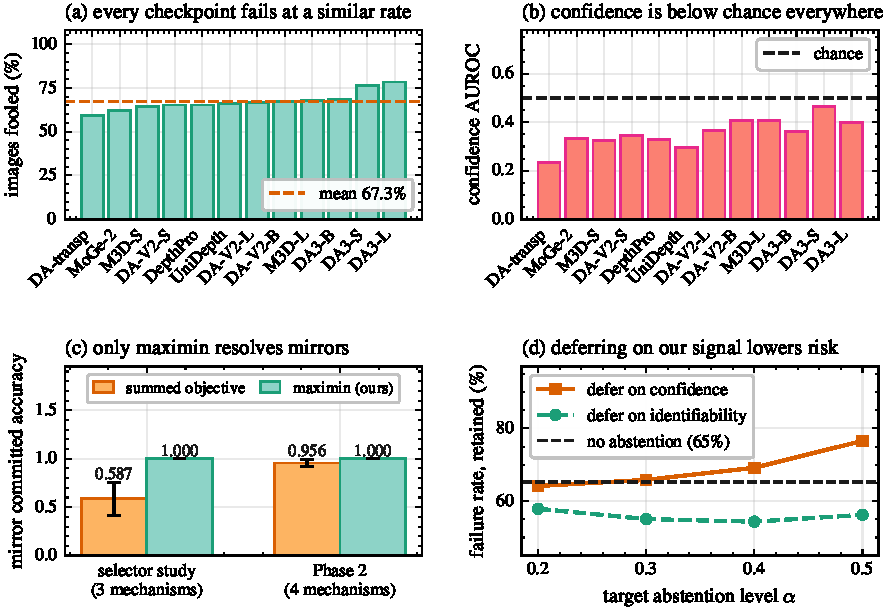
\includegraphics[width=\linewidth]{figures/fig_main.pdf}
\end{center}
\caption{\textbf{Headline results across the thirteen checkpoints.} (a) Images fooled. (b) Confidence
AUROC. (c) Committed accuracy on mirrors. (d) Split-conformal selective risk.}
\label{fig:main}
\end{figure}

We evaluate thirteen published checkpoints spanning seven architecture families and a
$38\times$ range in parameter count, all as released
\citep{depthanything2024,da3_2025,depthpro2025,moge2025,moge3_2026,metric3d2023,unidepth2024,unidepthv2_2025}
(Figure~\ref{fig:main}a,b). Every checkpoint fails on $59.5$ to $78.4\%$ of admissible
images, with the newest family among the most affected. On none of them does a confidence
proxy taken from the output of the predictor rise above chance at predicting its own
failure, with values from $0.234$ to $0.465$, whereas identifiability ranges from $0.467$
to $0.719$ and exceeds confidence on all thirteen. Calibration cannot repair a signal
ordered against the quantity of interest. Both signals meet split-conformal coverage at all
five levels, and yet deferring on confidence leaves a retained set failing at $76.6\%$
against a base rate of $65.2\%$, where identifiability lowers the same quantity to $54.4\%$
(Figure~\ref{fig:main}d). The criterion of Section~\ref{sec:real-protocol} excludes $159$ of
$455$ images whose stereo reference locks onto displayed content, which identifies
undecidable cases and removes them from scoring. Beyond this benchmark, two independent labels
agree. Accuracy split by the per-point layer index of a second benchmark reaches $0.848$
against $0.737$, and Table~\ref{tab:mirrors} repeats the evaluation on $123$ photographs of
\emph{real mirrors} whose contact geometry carries an independent annotation
\citep{mirror3d2021}. The same thirteen checkpoints report the depicted scene at $67.0\%$
there, against $66.8\%$ on displays, with relative error inside the mirror region reaching
$5.47\times$ the error outside and up to two thirds of frames placing the first surface
behind the glass. A different optical mechanism, annotated by a different group against a
human-placed plane rather than a stereo reference, therefore produces the same rate. Neither
label shares any machinery with a measure defined in Section~\ref{sec:method}.
\subsection{Qualitative and Error Analysis}
\label{sec:res-qualitative}
\begin{table}[t]
\caption{\textbf{Failure concentrates where the executed action separates the hypotheses least.} The
three categories of the illusion benchmark \citep{illusion2025}, over thirteen checkpoints.}
\label{tab:category}
\begin{center}
\footnotesize
\setlength{\tabcolsep}{4.2pt}
\begin{tabular}{lccccccc}
\toprule
\textbf{Category} & \textbf{Img.} & \textbf{Fooled} & \textbf{Range} &
\textbf{At $100\%$} & \textbf{Err in/out} & \textbf{Med.\ $\Delta$} &
\textbf{$\Delta < \epsilon$} \\
\midrule
Printed sheet on a table & $97$ & $43.0\%$ & $23.7$--$76.3$ & $0/13$ & $0.91\times$ & $1.07$ & $82.5\%$ \\
Poster beside an object & $104$ & $58.9\%$ & $34.6$--$75.0$ & $0/13$ & $1.23\times$ & $0.57$ & $86.5\%$ \\
Monitor in the frame & $95$ & $\mathbf{99.9\%}$ & $98.9$--$100$ & $\mathbf{12/13}$ & $2.62\times$ & $\mathbf{0.25}$ & $\mathbf{100\%}$ \\
\midrule
\textbf{All admissible} & $\mathbf{296}$ & $\mathbf{66.8\%}$ & $59.5$--$78.4$ & --- & $1.66\times$ & $0.45$ & $89.5\%$ \\
\bottomrule
\end{tabular}
\end{center}
\end{table}
Figure~\ref{fig:model-grid} places all thirteen checkpoints on one photograph of a poster
beside a window frame, where the stereo reference reports a near planar surface across the
outlined region and every checkpoint instead reports the structure painted on the poster.

\begin{wrapfigure}[16]{r}{0.42\textwidth}
\vspace{-0.9\baselineskip}
\centering
\includegraphics[width=0.40\textwidth]{figures/fig_model_grid.pdf}
\caption{\textbf{Every checkpoint reports the poster instead of the panel.} Inside the
outlined region each one errs by $1.1$ to $7.2$ times the error it makes outside.}
\label{fig:model-grid}
\end{wrapfigure}
The failure stays local to that region, at $1.1$ to $7.2$ times the error each checkpoint
makes outside. The aggregate rate above averages over three conditions that behave
differently, and Table~\ref{tab:category} separates them. On the $97$ images of a sheet lying on a table,
failure remains a minority outcome at $43.0\%$, the median separability of $1.07$~px clears
the threshold, and the relative error inside the ambiguous region stays below the error
outside that region at $0.91\times$. On the $95$ images containing a monitor, failure
becomes total, with twelve of the thirteen checkpoints failing on \emph{every} image, a
relative error of $2.62\times$ inside the region, a median separability of $0.25$~px, and
every image falling below $\epsilon$. Failure therefore concentrates exactly where the executed
action separates the two hypotheses least, which is the pattern predicted by the criterion of
Section~\ref{sec:separability}.

\begin{wrapfigure}[16]{r}{0.42\textwidth}
\vspace{-0.9\baselineskip}
\centering
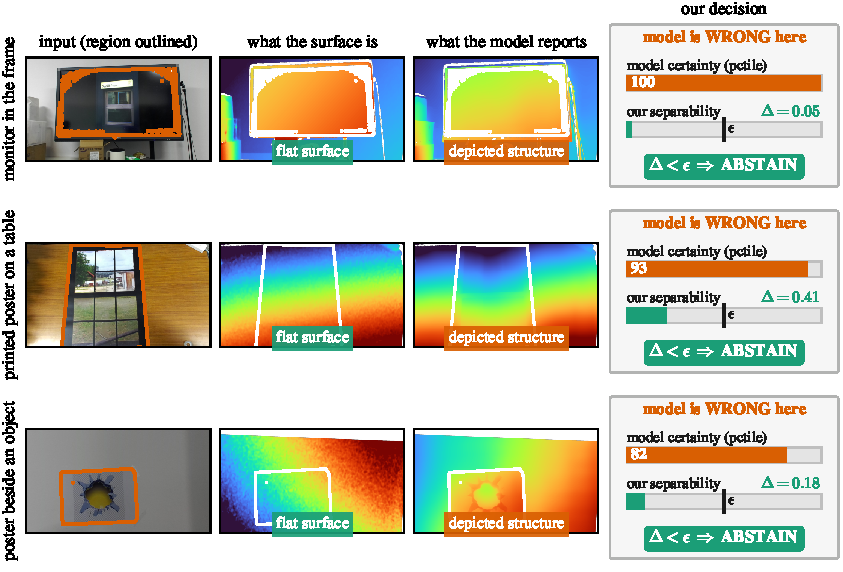
\includegraphics[width=0.40\textwidth]{figures/fig_qualitative.pdf}
\caption{\textbf{Three photographs, with the reference surface beside each prediction.}
Every prediction recovers the depicted scene rather than the panel.}
\label{fig:qualitative}
\end{wrapfigure}
Figure~\ref{fig:qualitative} presents three images with their predictions, namely a monitor
in the frame, a sheet lying on a table, and a poster beside an object. In each case the
reference geometry contains a flat panel across the annotated region, and the prediction
follows the scene painted on that panel. The top row carries the most confident prediction
among all $296$ images, which places the largest confidence of the evaluated set on a surface
that a hand would meet at the panel. Separability falls below $\epsilon$ in all three cases,
and \eqref{eq:abstain} therefore declines to answer where the predictor commits.

The residual errors of the proposed decision follow the same geometry. Where a sheet lies at an oblique
angle and the executed baseline moves across that obliquity, separability rises above
$\epsilon$, the system commits, and the commitment agrees with the reference. Where the
panel fills the frame and the stereo baseline shifts along the plane of the panel, no
hypothesis leaves a photometric trace, and the abstention that follows records the absence
of evidence rather than a mechanism.

\needspace{14\baselineskip}
\begin{wrapfigure}[12]{r}{0.42\textwidth}
\vspace{-0.8\baselineskip}
\centering
\includegraphics[width=0.40\textwidth]{figures/fig_delta_transfer.pdf}
\caption{Separability from one checkpoint predicts the failures of a \emph{different}
checkpoint, over $156$ ordered pairs.}
\label{fig:delta-transfer}
\vspace{-0.8\baselineskip}
\end{wrapfigure}
\paragraph{What Separability Measures.} Both hypotheses come from the output of the
predictor itself, and a direct control therefore tests whether the quantity describes the
scene or that one network (Figure~\ref{fig:delta-transfer}). Scoring the separability of
one checkpoint against the failures of a \emph{different} checkpoint, over all $156$ ordered
pairs, reaches $\mathbf{0.637}$, above chance on every pair and above the $0.597$ that each
checkpoint attains on its own failures. Idiosyncrasy does not transfer across networks,
whereas scene structure does, and a separability built from one predictor therefore carries
information about the scene rather than about the habits of that predictor.

\subsection{Choosing Where to Look on Real Photographs}
\label{sec:res-viewpoint}

The benchmark photographs each static scene from several camera positions, and the median
stereo disparity differs across frames while the scene does not, which is what a moved
observer produces. Fifty-five scenes therefore offer a real action set of three or more
viewpoints. Applying \eqref{eq:evidence-selection} and measuring error inside the ambiguous
region, which makes the outcome independent of every other part of the image, the
best-explained viewpoint lowers that error by $\mathbf{31.3\%}$ against a random choice, on
$\mathbf{13}$ of $13$ checkpoints, and the fooled rate falls from $48.0\%$ to $44.1\%$, on
$9$ of $13$. Real images carry no mechanism annotation, and this experiment therefore
measures error at the chosen viewpoint.

\subsection{Abstention from the Frozen Features of the Predictor}
\label{sec:res-learned}

The signals above are hand-designed, which raises the question of whether a learned
combination performs better and whether the learned quantity remains specific to one
predictor. Under the leave-one-model-out protocol, a gradient-boosted policy trained on
twelve checkpoints and tested on the thirteenth reaches $\mathbf{0.881}$ against $0.768$
for the strongest single feature, ahead on $\mathbf{13}$ of $13$. Moreover, on a single
checkpoint a head over \emph{frozen} encoder features reaches $\mathbf{0.887}$ out of fold,
with the layer chosen on inner folds and consistently an early one. No parameter of the
encoder changes, and the gate therefore adds no retraining and no architectural change. In
practice, answering the most confident $70\%$ of inputs lowers the failure rate from
$65.2\%$ to $50.2\%$, and answering half lowers the same rate to $37.8\%$, with every
threshold taken from out-of-fold scores under folds split by scene.

%============================================================================
% RELATED WORK
%============================================================================
\section{Related Work}
\label{sec:related}

Prior work localizes mirrors and glass as scene elements in their own right
\citep{mirrornet2019,glassdetection2020,mirror3d2021}, models transparency through
decomposed radiance \citep{glint2026}, and quantifies the difficulty with dedicated
benchmarks \citep{booster2023,clearpose2022,dreds2022}. Multi-layer formulations then
represent more than one surface along a ray
\citep{layereddepth2025,seegroup2026,depthfocus2026}, and an illusion benchmark documents at
scale that predictors report depicted rather than physical structure \citep{illusion2025}.
The present work steps back from recovering that geometry and asks first whether the
available observations determine the mechanism behind an appearance.

Classical analyses establish that image evidence alone can leave a family of scenes
indistinguishable \citep{belhumeur1999basrelief,sturm1997critical,oren1997theory,kutulakos2008theory},
while active and next-best-view perception selects viewpoints by a belief-weighted sum over
competing possibilities \citep{nbvreflective2022,rainforth2024}. We ask instead whether any
view within a bounded action set licenses a commitment, and we borrow the maximin criterion
that optimal design calls $T$-optimality
\citep{atkinson1975design,hunter1965experimental} together with the interventional framing
of causal identifiability \citep{citris2022}. Deferral rules \citep{chow1970,geifman2017,selectivenet2019}
and split conformal prediction \citep{vovk2005,lei2018} constrain how many predictions a
system retains rather than which ones, and a calibrated procedure therefore inherits the
ranking of the score that the procedure wraps.

%============================================================================
% CONCLUSION
%============================================================================
\section{Conclusion}
\label{sec:conclusion}

The present work asks whether a physical explanation is recoverable before asking what that
explanation is, and the measurements support that order. On the synthetic benchmark, whose
competing mechanisms are matched at the reference view, a single-view classifier stays at
exactly chance in every seed, abstention lowers false physical certainty from $0.832$ to
$0.000$, and selecting the action that separates the weakest contending pair reaches a
committed accuracy of $1.000$ on all four mechanisms. On real photographs, thirteen
checkpoints across seven architecture families report the depicted scene on $59.5$ to
$78.4\%$ of images, their confidence stays below chance at predicting these errors, and
split conformal prediction meets its coverage guarantee while retaining a set that fails
more often than answering everywhere. Three further measurements indicate where the missing
evidence can come from. The layer labels of an independent benchmark yield $0.848$ against
$0.737$, the best-explained viewpoint lowers ambiguous-region error by $31.3\%$ on every
checkpoint, and a gate over frozen encoder features reaches $0.887$ out of fold across all
thirteen unseen architectures, lowering the failure rate from $65.2\%$ to $50.2\%$ at $70\%$
coverage while the predictor itself receives no modification.

\paragraph{Limitations.} Separability requires an executed action, and a system that cannot
move gains nothing from the criterion developed here. The hypothesis family covers planar
optics, which keeps every transition closed form and the counterfactuals matched, and
curved mirrors together with thick glass therefore fall outside the present scope. On real
photographs the action set holds a single calibrated stereo baseline, and that experiment
consequently measures error at the chosen viewpoint rather than a recovered mechanism,
because real images carry no mechanism annotation. Appendix~\ref{sec:supp-limits} states
the remaining limitations in full, and Appendix~\ref{sec:supp-extension} describes the
route beyond planar optics.


\bibliography{iclr2027_conference}
\bibliographystyle{iclr2027_conference}

%============================================================================
% SUPPLEMENTARY MATERIAL
%============================================================================
\clearpage
\clearpage
\appendix
\section*{Supplementary Material}

% The appendix carries its own contents list. Entries destined for the table of
% contents are diverted into \jobname.stoc from this point on, so the list can
% only ever hold appendix material and nothing in the main text needs
% suppressing. Captions write to .lof and .lot and are passed through unchanged,
% otherwise every figure and table would be listed here as well.
\makeatletter
\let\supp@addcontentsline\addcontentsline
\def\supp@toc{toc}
\renewcommand\addcontentsline[3]{%
  \begingroup
    \def\supp@arg{#1}%
    \ifx\supp@arg\supp@toc
      \endgroup\supp@addcontentsline{stoc}{#2}{#3}%
    \else
      \endgroup\supp@addcontentsline{#1}{#2}{#3}%
    \fi}
\begingroup
  \renewcommand{\contentsname}{\normalsize Contents}
  \setlength{\parskip}{0pt}
  \setcounter{tocdepth}{2}
  \footnotesize
  \section*{\contentsname}
  \@starttoc{stoc}
\endgroup
\makeatother
\bigskip


Every number reported here comes from the same runs as the main paper. No part of this
appendix revises a result of Section~\ref{sec:results}, and the tables below extend those
results with the remaining metrics, the per-family breakdown, and the analytical component
that space kept out of the main text.

\section{The Method in Detail}

\subsection{Why One Image Admits Several Mechanisms}
\label{sec:supp-concept}

Figure~\ref{fig:concept} presents the premise of the paper in one picture, namely three
physical arrangements that produce the same image, together with the effect that an
executed motion has on each arrangement.

\begin{figure}[!ht]
\begin{center}
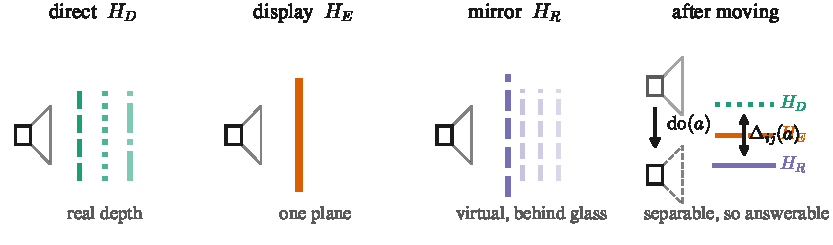
\includegraphics[width=0.92\linewidth]{figures/fig_concept.pdf}
\end{center}
\caption{\textbf{One image admits three mechanisms, and motion tells them apart.} The colored plane
marks the surface a hand would touch in each arrangement.}
\label{fig:concept}
\end{figure}

\subsection{The Decision Pipeline}
\label{sec:supp-pipeline}

Figure~\ref{fig:pipeline} sets out how the pieces of Section~\ref{sec:method} compose into a
single decision.

\begin{figure}[!ht]
\begin{center}
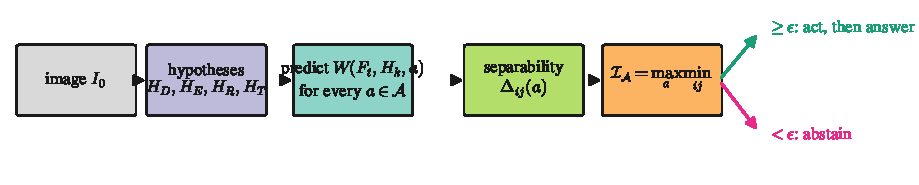
\includegraphics[width=0.96\linewidth]{figures/fig_pipeline.pdf}
\end{center}
\caption{\textbf{The pieces compose into a single decision.} The system acts only when identifiability
clears the perceptual threshold, and declines to answer otherwise.}
\label{fig:pipeline}
\end{figure}

\subsection{The Real-Photograph Protocol in Detail}
\label{sec:supp-protocol}

Figure~\ref{fig:supp-protocol} presents the construction of the real-data measurement and
the place where we fit each quantity. A physical sheet or panel is flat, and reference
disparity inside the annotated region should therefore stay planar. Where planarity fails,
the stereo reference has locked onto displayed content rather than onto the panel and cannot
settle what the predictor reported, and we therefore retain an image only when a plane
fitted to that disparity attains $R^2 \geq 0.90$. We report the number of images that this
rule excludes.

\begin{figure}[!ht]
\begin{center}
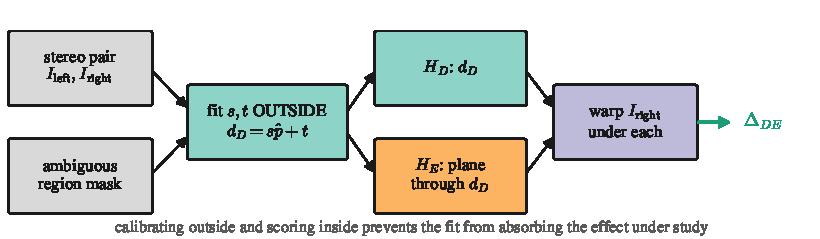
\includegraphics[width=\linewidth]{figures/fig_supp_protocol.pdf}
\end{center}
\caption{\textbf{How the real-data measurement is built.} Comparing two warps of the same photograph
cancels illumination, sensor noise, and rectification error.}
\label{fig:supp-protocol}
\end{figure}

\subsection{Minimum Causal Resolving Baseline}
\label{sec:supp-mcrb}

\begin{proposition}[Minimum causal resolving baseline]\label{prop:mcrb}
Consider the pair $(H_D, H_E)$ under a pure lateral translation of baseline $B$,
with a pinhole camera of horizontal focal length $f$ pixels, and $B \ll Z$. Two
scene points at depths $Z_1 \neq Z_2$ then shift by approximately $fB/Z_i$ and
therefore produce a differential parallax $fB\,|1/Z_1 - 1/Z_2|$, whereas a static planar
display produces none once the screen-plane homography is compensated. Requiring
that differential parallax to exceed the perceptual threshold $\delta$ yields the
smallest resolving baseline
\begin{equation}
\label{eq:mcrb}
B_{\min} \;>\; \frac{\delta}{f\left|1/Z_1 - 1/Z_2\right|},
\end{equation}
where $\delta$ coincides with $\epsilon$ whenever the motion term dominates the composite
distance of \eqref{eq:distance}.
\end{proposition}

The hypotheses of Proposition~\ref{prop:mcrb} are restrictive, and we check them before
evaluating \eqref{eq:mcrb}, therefore a violated assumption yields a missing prediction
rather than a number. The proposition covers neither view-tracked displays, which no
baseline resolves, nor mirrors, whose virtual scene carries genuine parallax.

\subsection{Notation}
\label{sec:supp-notation}

The formulation moves between three levels, and Table~\ref{tab:supp-notation} fixes which
symbol belongs to which level. Landmarks carry image coordinates and depths, and the
composite distance of \eqref{eq:distance} operates over those landmarks, whereas the
photometric separability of \eqref{eq:delta-photometric} compares warped images, which
explains why one quantity appears in pixels and the other in intensity units.

\begin{table}[!ht]
\caption{\textbf{The symbols used throughout the paper.} Each one belongs to the image level, the
landmark level, the hypothesis level, the action level, or the belief level.}
\label{tab:supp-notation}
\begin{center}
\footnotesize
\begin{tabular}{lll}
\toprule
\textbf{Symbol} & \textbf{Level} & \textbf{Meaning} \\
\midrule
$I_0$, $C_0$ & image & reference image and the pose of that image \\
$E$, $F_0 = E(I_0)$ & landmarks & perception encoder and the reported geometry \\
$H_D, H_E, H_R, H_T$ & hypothesis & direct, emissive panel, planar mirror, planar slab \\
$a \in \mathcal{A}$ & action & a rigid camera motion; $|\mathcal{A}| = 33$ synthetically \\
$W$, $\hat{F}^{\,k,a}$ & landmarks & transition, and what $H_k$ predicts after $a$ \\
$D$ & landmarks & composite distance of \eqref{eq:distance}, in pixels \\
$\Delta_{ij}(a)$ & landmarks & separability of $H_i$ and $H_j$ under $a$ \\
$\mathcal{I}_{\mathcal{A}}$ & landmarks & identifiability, the best $\Delta$ over $\mathcal{A}$ \\
$\epsilon$ & landmarks & perceptual threshold, $1.0$~px \\
$d_D$, $d_E$ & image & disparity each hypothesis predicts, \eqref{eq:align} \\
$R_k$ & image & the second view warped under $H_k$, \eqref{eq:warp} \\
$\Delta_{DE}$ & image & photometric separability, in intensity units \\
$p_t(H_k)$, $\beta$, $\tau$ & belief & posterior, inverse temperature, commitment threshold \\
\bottomrule
\end{tabular}
\end{center}
\end{table}

\subsection{Metric Definitions}
\label{sec:supp-metrics}

Table~\ref{tab:supp-metrics} defines the metrics used throughout. The unresolvable
configurations that Section~\ref{sec:setup} retains take two forms, namely view-tracked
displays observed within their aperture, which no baseline resolves, and mirrors arranged to
mimic an opening of the same shape.

\begin{table}[!ht]
\caption{\textbf{The metrics reported throughout the paper.} Here $\hat{H}$ denotes the predicted
mechanism, $H^\star$ the true one, and $y_{\mathrm{id}} = 0$ a case that no action resolves.}
\label{tab:supp-metrics}
\begin{center}
\footnotesize
\begin{tabular}{llp{6.0cm}}
\toprule
\textbf{Metric} & \textbf{Definition} & \textbf{Question answered} \\
\midrule
CEA & $P(\hat{H} = H^\star)$ & how often the mechanism is named correctly, abstention counted as an error \\
Committed acc. & $P(\hat{H} = H^\star \mid \text{answered})$ & how often a given answer is correct \\
Abstention rate & $P(\text{abstain})$ & how often an answer is withheld \\
FPCR & $P(\max_k p(H_k) > \tau \mid y_{\mathrm{id}} = 0)$ & how often a confident answer is given where none is warranted \\
Ident.\ AUROC & predicted against true resolvability & whether unresolvable cases are recognized \\
Normalized regret & chosen against best available action & whether a near-optimal intervention was selected \\
Motion cost & translation plus weighted rotation & how much movement the decision required \\
\bottomrule
\end{tabular}
\end{center}
\end{table}

\section{The Synthetic Benchmark}

\subsection{Choosing the Intervention, in Full}
\label{sec:supp-phase2}

Figure~\ref{fig:main}c plots the mirror comparison quoted in Section~\ref{sec:res-synth},
and Table~\ref{tab:phase2} reports every objective on both studies.

\begin{table}[!ht]
\caption{\textbf{Maximin selection resolves mirrors where a summed objective does not.} Eleven seeds
per study, where chance stands at $0.250$ over the four mechanisms.}
\label{tab:phase2}
\begin{center}
\footnotesize
\begin{tabular}{lccccc}
\toprule
& \multicolumn{2}{c}{\textbf{Mirror committed}} &
\multicolumn{3}{c}{\textbf{Phase~2, four mechanisms}} \\
\cmidrule(lr){2-3}\cmidrule(lr){4-6}
\textbf{Objective} & selector study & Phase~2 & committed & abstains & forced CEA \\
\midrule
Single-view classifier & --- & --- & $0.250{\pm}0.000$ & $0\%$ & $0.250{\pm}0.000$ \\
Passive multi-view     & --- & --- & $0.510{\pm}0.020$ & $0\%$ & $0.510{\pm}0.020$ \\
Max-baseline           & --- & $0.925{\pm}0.048$ & $0.981{\pm}0.011$ & $73\%$ & --- \\
Summed \eqref{eq:sum}  & $0.587{\pm}0.164$ & $0.956{\pm}0.035$ & $0.986{\pm}0.010$ & $69\%$ & --- \\
\textbf{Maximin} \eqref{eq:maximin} & $\mathbf{1.000{\pm}0.000}$ & $\mathbf{1.000{\pm}0.000}$ & $\mathbf{1.000{\pm}0.000}$ & $72\%$ & $\mathbf{0.808{\pm}0.023}$ \\
\bottomrule
\end{tabular}
\end{center}
\end{table}

\subsection{Calibrated Deferral and Imperfect Execution}
\label{sec:supp-noise}

Table~\ref{tab:noise} reports the effect of executing a chosen action imperfectly on the
synthetic benchmark, and Table~\ref{tab:conformal} reports split-conformal deferral on the
real benchmark.

\begin{table}[!ht]
\caption{\textbf{A large separability margin absorbs imperfect execution.} Under $\pm 1$~cm and
$\pm 0.5^{\circ}$ of error, the hypothesis-blind proxy loses half its accuracy and ours
$2.9\%$.}
\label{tab:noise}
\begin{center}
\footnotesize
\begin{tabular}{lcccc}
\toprule
\textbf{Method} & \textbf{Clean CEA} & \textbf{Perturbed CEA} & \textbf{Change} & \textbf{$t$} \\
\midrule
Passive multi-view (does not act) & $0.621$ & $0.621$ & $+0.0\%$ & --- \\
Generic next-best-view proxy   & $0.371$ & $0.192$ & $-48.4\%$ & $-14.05$ \\
Random intervention & $0.409$ & $0.291$ & $-29.0\%$ & $-10.64$ \\
Max-baseline        & $0.502$ & $0.478$ & $-4.7\%$  & $-3.68$ \\
\textbf{Ours}       & $0.560$ & $0.544$ & $\mathbf{-2.9\%}$ & $-3.05$ \\
\bottomrule
\end{tabular}
\end{center}
\end{table}

\begin{table}[!ht]
\caption{\textbf{Coverage holds for both signals, while only identifiability lowers risk.}
Split-conformal deferral over $296$ images, at four target levels.}
\label{tab:conformal}
\begin{center}
\footnotesize
\begin{tabular}{lccccccc}
\toprule
& & \multicolumn{4}{c}{\textbf{Failure rate among retained images}} & & \\
\cmidrule(lr){3-6}
\textbf{Deferral signal} & \textbf{AUROC} & $\alpha{=}0.2$ & $\alpha{=}0.3$ &
$\alpha{=}0.4$ & $\alpha{=}0.5$ & \textbf{Coverage} & \textbf{Best gain} \\
\midrule
No abstention            & ---     & \multicolumn{4}{c}{$65.2\%$} & --- & --- \\
Confidence, augmented & $0.339$ & $64.2\%$ & $65.8\%$ & $69.2\%$ & $76.6\%$ & $5/5$ & $-1.0$ \\
\textbf{Identifiability} & $\mathbf{0.645}$ & $58.1\%$ & $54.7\%$ & $\mathbf{53.1\%}$ & $55.0\%$ & $5/5$ & $\mathbf{-12.1}$ \\
\bottomrule
\end{tabular}
\end{center}
\end{table}

\section{Real Photographs}

\subsection{Per-Checkpoint Results}
\label{sec:supp-models}

Table~\ref{tab:models} lists the per-checkpoint values summarized in
Section~\ref{sec:res-universal} for the released checkpoints
\citep{depthanything2024,da3_2025,depthpro2025,moge2025,moge3_2026,metric3d2023,unidepth2024,unidepthv2_2025},
together with parameter counts and family membership, while Figure~\ref{fig:model-grid} of
the main text places all thirteen checkpoints on a single photograph.

\begin{table}[!ht]
\caption{\textbf{Every published checkpoint fails, and none of them anticipates its own failure.}
Confidence takes the better of raw confidence and a four-member ensemble.}
\label{tab:models}
\begin{center}
\footnotesize
\begin{tabular}{llrccc}
\toprule
\textbf{Checkpoint} & \textbf{Family} & \textbf{Params} & \textbf{Fooled} &
\textbf{Conf.\ AUROC} & \textbf{Ident.\ AUROC} \\
\midrule
DA-V2-Small     & Depth-Anything-V2 & $24.8$M  & $65.2\%$ & $0.344$ & $0.645$ \\
DA-V2-Base      & Depth-Anything-V2 & $97.5$M  & $67.2\%$ & $0.408$ & $0.588$ \\
DA-V2-Large     & Depth-Anything-V2 & $335.3$M & $66.6\%$ & $0.367$ & $0.467$ \\
DA-transparency & Depth-Anything-V2 & $24.8$M  & $\mathbf{59.5\%}$ & $\mathbf{0.234}$ & $0.719$ \\
DA3-Small       & Depth-Anything-3  & $24.8$M  & $76.4\%$ & $0.465$ & $0.479$ \\
DA3-Base        & Depth-Anything-3  & $97.5$M  & $68.2\%$ & $0.362$ & $0.576$ \\
DA3-Large       & Depth-Anything-3  & $410.9$M & $\mathbf{78.4\%}$ & $0.399$ & $0.512$ \\
DepthPro        & DepthPro          & $952.0$M & $65.2\%$ & $0.328$ & $0.659$ \\
MoGe-2          & MoGe-2            & $330.9$M & $62.2\%$ & $0.334$ & $0.642$ \\
MoGe-3-ViT-L    & MoGe-3            & $330.9$M & $61.8\%$ & $0.360$ & $0.595$ \\
Metric3D-Small  & Metric3D          & $37.5$M  & $64.5\%$ & $0.323$ & $0.593$ \\
Metric3D-Large  & Metric3D          & $343.0$M & $67.6\%$ & $0.406$ & $0.593$ \\
UniDepth-v2     & UniDepth          & $353.8$M & $66.2\%$ & $0.295$ & $0.692$ \\
\midrule
\emph{range} & \emph{7 families} & $38\times$ & $59.5$--$78.4\%$ & $0.234$--$0.465$ & $0.467$--$0.719$ \\
\bottomrule
\end{tabular}
\end{center}
\end{table}

\subsection{Extended Results by Architecture Family}
\label{sec:supp-family}

Table~\ref{tab:supp-family} and Figure~\ref{fig:supp-extended} average within architecture
family, which confirms that a single lineage does not drive the pattern.

\begin{figure}[!ht]
\begin{center}
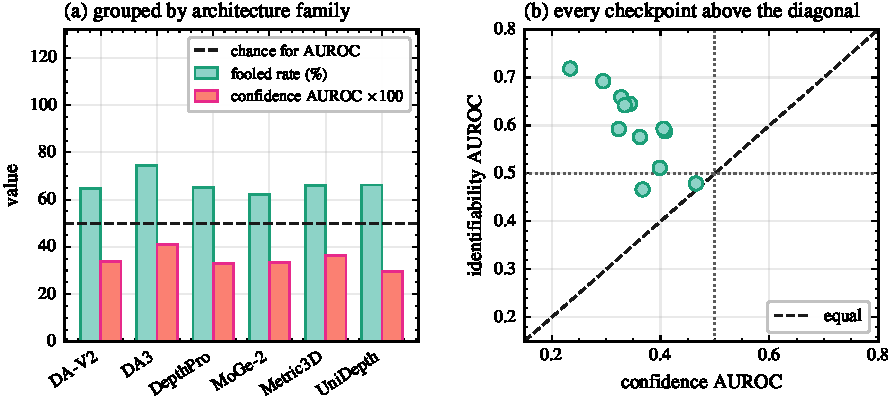
\includegraphics[width=\linewidth]{figures/fig_supp_extended.pdf}
\end{center}
\caption{\textbf{Two views of Table~\ref{tab:models}.} (a) Mean confidence AUROC by architecture
family. (b) Identifiability against confidence, one point per checkpoint.}
\label{fig:supp-extended}
\end{figure}

\begin{table}[!ht]
\caption{\textbf{No single lineage drives the pattern.} Every architecture family fails on roughly two
images in three and stays below chance in mean confidence AUROC.}
\label{tab:supp-family}
\begin{center}
\footnotesize
\begin{tabular}{lcccc}
\toprule
\textbf{Family} & \textbf{Ckpts} & \textbf{Mean fooled} &
\textbf{Mean conf.} & \textbf{Mean ident.} \\
\midrule
Depth-Anything-V2 & $4$ & $64.6\%$ & $0.338$ & $0.605$ \\
Depth-Anything-3  & $3$ & $74.3\%$ & $0.409$ & $0.522$ \\
DepthPro          & $1$ & $65.2\%$ & $0.328$ & $0.659$ \\
MoGe-2            & $1$ & $62.2\%$ & $0.334$ & $0.642$ \\
MoGe-3            & $1$ & $61.8\%$ & $0.360$ & $0.595$ \\
Metric3D          & $2$ & $66.0\%$ & $0.365$ & $0.593$ \\
UniDepth          & $1$ & $66.2\%$ & $0.295$ & $0.692$ \\
\midrule
\textbf{All} & $\mathbf{13}$ & $\mathbf{66.8\%}$ & $\mathbf{0.356}$ & $\mathbf{0.597}$ \\
\bottomrule
\end{tabular}
\end{center}
\end{table}

\subsection{Per-Category Behavior on the Illusion Benchmark}
\label{sec:supp-category}

The aggregate error ratio quoted in Section~\ref{sec:res-universal} resolves into three
categories that behave differently, as Table~\ref{tab:supp-category} reports.

\begin{table}[!ht]
\caption{\textbf{The penalty grows largest where a monitor occupies the frame.} Admissible images by
category of the illusion benchmark \citep{illusion2025}.}
\label{tab:supp-category}
\begin{center}
\footnotesize
\begin{tabular}{lcccc}
\toprule
\textbf{Category} & \textbf{Images} & \textbf{Error ratio in/out} &
\textbf{Fooled} & \textbf{Ref.\ planarity} \\
\midrule
Printed sheet on a table & $97$ & $0.78\times$ & $33\%$ & $0.99$ \\
Poster beside an object  & $104$ & $1.47\times$ & $63\%$ & $0.99$ \\
Monitor in the frame & $95$ & $\mathbf{2.23\times}$ & $\mathbf{100\%}$ & $0.99$ \\
\midrule
\textbf{All admissible}  & $\mathbf{296}$ & $\mathbf{1.42\times}$ & $\mathbf{65.2\%}$ & $\mathbf{0.989}$ \\
\bottomrule
\end{tabular}
\end{center}
\end{table}

\subsection{Choosing Where to Look}
\label{sec:supp-viewpoint}

Table~\ref{tab:supp-viewpoint} reports the full comparison. Fifty-five scenes without video
content offer three or more camera positions of the same static content. We exclude video
scenes because their frames differ by displayed content rather than by observer position,
and treating those frames as an action set would count a change of stimulus as a change of
viewpoint.

\begin{table}[!ht]
\caption{\textbf{The best-explained viewpoint lowers error inside the ambiguous region.} Thirteen
checkpoints over $55$ scenes, against a random choice of viewpoint.}
\label{tab:supp-viewpoint}
\begin{center}
\footnotesize
\begin{tabular}{lcc}
\toprule
\textbf{Viewpoint chosen by} & \textbf{Error inside region} & \textbf{Fooled} \\
\midrule
first frame, no choice          & $0.0671$ & $48.7\%$ \\
uniformly at random             & $0.0591$ & $48.0\%$ \\
the predictor's own confidence  & $0.0439$ & $46.4\%$ \\
\textbf{best-explained observation} \eqref{eq:evidence-selection} & $\mathbf{0.0406}$ & $\mathbf{44.1\%}$ \\
\midrule
\multicolumn{3}{l}{\emph{ahead of a random choice on $13/13$ checkpoints by error, $9/13$ by fooled rate}} \\
\bottomrule
\end{tabular}
\end{center}
\end{table}

\subsection{Second Dataset with Ordinal Supervision}
\label{sec:supp-layered}

The second dataset provides ordinal relations between point pairs rather than dense depth,
together with a per-point layer index authored independently of the present work.

\begin{table}[!ht]
\caption{\textbf{An independent layer annotation separates the same failure.} LayeredDepth
validation \citep{layereddepth2025}, where both architectures fall behind through glass.}
\label{tab:supp-layered}
\begin{center}
\footnotesize
\begin{tabular}{lccccc}
\toprule
\textbf{Checkpoint} & \textbf{Single-layer} & \textbf{Multi-layer} &
\textbf{Gap} & \textbf{First surface} & \textbf{Through glass} \\
\midrule
DA-V2-Small & $0.848$ & $0.737$ & $\mathbf{+0.111}$ & $0.847$ & $0.784$ \\
DepthPro    & $0.843$ & $0.669$ & $\mathbf{+0.175}$ & $0.842$ & $0.741$ \\
\bottomrule
\end{tabular}
\end{center}
\end{table}

\subsection{Real Mirrors, with Annotated Contact Geometry}
\label{sec:supp-mirrors}

Every real-photograph result in the main text concerns physical sheets and panels, because
the real split of the illusion benchmark contains no photograph of a physical mirror, and
reflection therefore appears there on synthetic data alone. The present section closes that
gap on real photographs, using mirror annotations produced by another group.

Mirror3D \citep{mirror3d2021} annotates real mirrors with an instance mask and a
three-dimensional mirror plane, layered on NYUv2 \citep{nyuv2_2012}, which requires no data
agreement. The annotated plane serves as the appropriate ground truth here precisely because
a depth sensor does not, since a structured-light sensor returns either no signal or
unreliable depth on a mirror, and the human-placed plane therefore remains the only
statement of where the first touchable surface lies. We apply the same discipline as in the
stereo protocol, fitting scale and shift outside the annotated region against reference
depth, applying them inside that region, and carrying out the comparison in inverse-depth
space, because the predictors return relative inverse depth rather than meters. The released
annotations carry a $5\%$ center crop, and we shift the principal point to match.

Table~\ref{tab:mirrors} in the main text reports the outcome over $123$ annotated frames for
the same thirteen checkpoints that the display benchmark uses, and the two results therefore
rest on one roster. Eleven of the thirteen lie between $62.6\%$ and $79.7\%$, around a mean
of $67.0\%$. Figure~\ref{fig:supp-mirrors} presents individual photographs from this set.

Two checkpoints stand apart at $41.5\%$, and we report them separately. The first is the
transparency fine-tuned variant, where training that targets one non-Lambertian mechanism
appears to transfer to another, and the same checkpoint fails least often on the display
benchmark at $59.5\%$. The second is Metric3D-Large, whose small counterpart fails on
$78.9\%$ of the same frames, while the two agree closely on displays at $64.5\%$ and
$67.6\%$, and the divergence therefore describes that checkpoint on this data rather than
the family, a difference we leave unexplained.

\begin{figure}[!ht]
\begin{center}
\includegraphics[width=\linewidth]{figures/fig_nyu_mirrors.pdf}
\end{center}
\caption{\textbf{A predictor places a mirror surface inside the reflected room.} The reported depth
reaches about twice the distance of the annotated plane, outlined in every panel.}
\label{fig:supp-mirrors}
\end{figure}

NYUv2 provides no camera poses and only accelerometer orientation, which leaves the action
set empty, and this experiment therefore tests neither separability nor viewpoint selection
nor abstention. The experiment establishes instead that the phenomenon formalized here
extends past displays and persists when an independent annotation, rather than a plane fit,
states where the physical surface lies.

\section{Learned Abstention}

\subsection{Learned Abstention, Summary}
\label{sec:supp-learned}

We pool the features over the ambiguous region as three contrasts, namely the difference
between the pooled representation inside and outside the region, the spread within the
region, and the difference between a one-token boundary ring and its surroundings, where the
mechanisms separate. Contrasts serve as inputs because a representation encoding ambiguity
should differ from its surroundings. We place tokens on the grid that the processor
produces, choose the layer on inner folds, and fit three classifier families, namely
$L_2$-regularized logistic regression, histogram gradient boosting, and \textsc{XGBoost},
which keeps any conclusion independent of one inductive bias. The boosted models stay at
depth $3$ with at least $40$ samples per leaf, because a few thousand rows from fewer than a
hundred scenes would otherwise be memorized. We also verify the depth convention of each
checkpoint against reference stereo disparity before use, because the attribute
conventionally named \texttt{predicted\_depth} carries metric depth in some families and
inverse depth in others, and an inverted convention would exchange near for far while still
producing plausible numbers.

Table~\ref{tab:supp-learned} presents the summary referenced from
Section~\ref{sec:res-learned} and Figure~\ref{fig:transfer} plots the transfer result, while
the next subsection expands the leave-one-model-out column to every one of the thirteen
held-out checkpoints.

\begin{table}[!ht]
\caption{\textbf{A learned policy predicts failure across held-out predictors.} Folds split by base
scene, which keeps frames of one scene inside a single partition.}
\label{tab:supp-learned}
\begin{center}
\footnotesize
\begin{tabular}{lccc}
\toprule
\textbf{Policy} & \textbf{Grouped CV} & \textbf{Nested CV} & \textbf{Leave-one-model-out} \\
\midrule
\multicolumn{4}{l}{\emph{all 13 checkpoints, 3{,}848 image--model pairs, 68 scenes}} \\
Strongest single feature    & $0.766$ & --- & $0.768$ \\
Logistic regression         & $0.755$ & $0.757$ & $0.779$ \\
\textsc{XGBoost}            & --- & $0.834$ & --- \\
Histogram gradient boosting & $\mathbf{0.834}$ & $\mathbf{0.831}$ & $\mathbf{0.881}$ ($13/13$) \\
\midrule
\multicolumn{4}{l}{\emph{single checkpoint, identical data for all three}} \\
Strongest single feature    & $0.819$ & --- & --- \\
Hand-designed features      & $0.858$ & --- & --- \\
\textbf{Frozen-encoder head} & $\mathbf{0.887}$ & --- & --- \\
\bottomrule
\end{tabular}
\end{center}
\end{table}

\begin{figure}[!ht]
\begin{center}
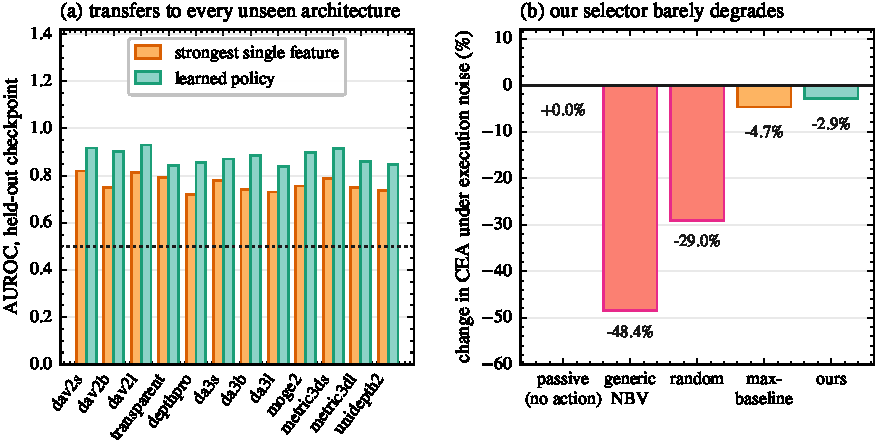
\includegraphics[width=\linewidth]{figures/fig_transfer.pdf}
\end{center}
\caption{\textbf{The learned policy transfers and the selection stays stable.} (a) Held-out
checkpoints against the strongest single feature. (b) Accuracy under imperfect execution.}
\label{fig:transfer}
\end{figure}

\subsection{Full Leave-One-Model-Out Results}
\label{sec:supp-lomo}

Table~\ref{tab:supp-lomo} expands the leave-one-model-out protocol of
Table~\ref{tab:supp-learned} to every held-out checkpoint, together with the regularization
sweep for the frozen-encoder head.

\begin{table}[!ht]
\caption{\textbf{The policy leads on every held-out checkpoint.} The upper block reaches a mean margin
of $+0.113$, and the lower block varies by $0.036$ across three decades of $C$.}
\label{tab:supp-lomo}
\begin{center}
\footnotesize
\begin{tabular}{lccc|lccc}
\toprule
\textbf{Held out} & \textbf{Learned} & \textbf{Baseline} & \textbf{$\Delta$} &
\textbf{Held out} & \textbf{Learned} & \textbf{Baseline} & \textbf{$\Delta$} \\
\midrule
DA-V2-Small     & $0.917$ & $0.819$ & $+0.098$ & DepthPro       & $0.855$ & $0.721$ & $+0.134$ \\
DA-V2-Base      & $0.900$ & $0.748$ & $+0.152$ & MoGe-2         & $0.906$ & $0.756$ & $+0.150$ \\
DA-V2-Large     & $0.932$ & $0.812$ & $+0.120$ & MoGe-3-ViT-L   & $0.904$ & $0.811$ & $+0.093$ \\
DA-transparency & $0.834$ & $0.791$ & $+0.043$ & Metric3D-Small & $0.915$ & $0.787$ & $+0.127$ \\
DA3-Small       & $0.871$ & $0.781$ & $+0.091$ & Metric3D-Large & $0.855$ & $0.750$ & $+0.105$ \\
DA3-Base        & $0.887$ & $0.739$ & $+0.148$ & UniDepth-v2    & $0.855$ & $0.738$ & $+0.117$ \\
DA3-Large       & $0.828$ & $0.731$ & $+0.097$ & & &  \\
\midrule
\multicolumn{8}{c}{\textbf{mean} $\;0.881$ against $0.768$, margin $+0.113$, ahead on $13/13$} \\
\midrule
\multicolumn{8}{l}{\emph{frozen-encoder head: AUROC against regularization strength $C$, grouped five-fold, one checkpoint}} \\
$C$ & $0.001$ & $0.005$ & $0.020$ & $0.100$ & $0.500$ & $2.000$ & $10.000$ \\
AUROC & $\mathbf{0.879}$ & $0.875$ & $0.873$ & $0.866$ & $0.859$ & $0.853$ & $0.843$ \\
\bottomrule
\end{tabular}
\end{center}
\end{table}

\subsection{Full Abstention Retention Curve}
\label{sec:supp-operating}

The main text quotes three operating points, and Table~\ref{tab:supp-operating} reports the
complete curve.

\begin{table}[!ht]
\caption{\textbf{Answering fewer inputs lowers the failure rate monotonically.} The frozen-encoder
gate on $296$ images from DA-V2-Small, against a base failure rate of $65.2\%$.}
\label{tab:supp-operating}
\begin{center}
\footnotesize
\begin{tabular}{lccc}
\toprule
\textbf{Inputs answered} & \textbf{Failure rate among them} &
\textbf{Change} & \textbf{Failures avoided} \\
\midrule
$100\%$ & $65.2\%$ & --- & $0$ \\
$90\%$  & $61.3\%$ & $-3.9$  & $30$ \\
$80\%$  & $56.5\%$ & $-8.7$  & $59$ \\
$70\%$  & $50.2\%$ & $-15.0$ & $89$ \\
$60\%$  & $43.3\%$ & $-21.9$ & $116$ \\
$50\%$  & $37.8\%$ & $-27.4$ & $137$ \\
$40\%$  & $29.7\%$ & $-35.5$ & $158$ \\
$30\%$  & $23.6\%$ & $-41.6$ & $172$ \\
\bottomrule
\end{tabular}
\end{center}
\end{table}

\section{Robustness and Controls}

\subsection{Threshold Sensitivity}
\label{sec:supp-sensitivity}

Three thresholds carry the decisions in this work, and the present section reports their
influence. Table~\ref{tab:supp-epsilon} sweeps the perceptual threshold,
Table~\ref{tab:supp-admissibility} sweeps the admissibility criterion, and
Table~\ref{tab:supp-category-exclusion} reports what that criterion removes by category. We
recompute every number below from the artifacts of the original runs, without re-executing
an experiment or redrawing a seed, and each row therefore records the decision that the same
system would have taken under a different threshold on identical data.

\begin{table}[!ht]
\caption{\textbf{The decision does not depend on where the threshold falls.} Sweeping $\epsilon$ from
$0.25$ to $3.0$~px over eleven seeds leaves every reported quantity unchanged.}
\label{tab:supp-epsilon}
\begin{center}
\footnotesize
\begin{tabular}{lcccc}
\toprule
$\epsilon$ (px) & \textbf{abstains} & \textbf{CEA} & \textbf{committed} & \textbf{FPCR} \\
\midrule
$0.25$ & $34.3\%$ & $0.560$ & $0.855$ & $0.000$ \\
$0.50$ & $34.3\%$ & $0.560$ & $0.855$ & $0.000$ \\
$0.75$ & $34.3\%$ & $0.560$ & $0.855$ & $0.000$ \\
\textbf{1.00} & $\mathbf{34.3\%}$ & $\mathbf{0.560}$ & $\mathbf{0.855}$ & $\mathbf{0.000}$ \\
$1.50$ & $34.3\%$ & $0.560$ & $0.855$ & $0.000$ \\
$2.00$ & $34.3\%$ & $0.560$ & $0.855$ & $0.000$ \\
$3.00$ & $34.3\%$ & $0.560$ & $0.855$ & $0.000$ \\
$5.00$ & $37.8\%$ & $0.539$ & $0.868$ & $0.000$ \\
\bottomrule
\end{tabular}
\end{center}
\end{table}

\begin{table}[!ht]
\caption{\textbf{The conclusions hold wherever the admissibility criterion falls.} Retaining $55\%$ to
$71\%$ of the benchmark moves the fooled rate by $1.6$ points.}
\label{tab:supp-admissibility}
\begin{center}
\footnotesize
\begin{tabular}{lcccc}
\toprule
$R^2$ threshold & \textbf{retained} & \textbf{fooled} & \textbf{ident.\ AUROC} & \textbf{region-size AUROC} \\
\midrule
$0.70$ & $70.5\%$ & $64.8\%$ & $0.641$ & $0.813$ \\
$0.80$ & $69.5\%$ & $65.2\%$ & $0.637$ & $0.820$ \\
$0.85$ & $67.7\%$ & $65.9\%$ & $0.637$ & $0.822$ \\
\textbf{0.90} & $\mathbf{65.1\%}$ & $\mathbf{65.2\%}$ & $\mathbf{0.645}$ & $0.819$ \\
$0.95$ & $63.1\%$ & $64.8\%$ & $0.656$ & $0.819$ \\
$0.98$ & $55.4\%$ & $64.3\%$ & $0.692$ & $0.827$ \\
\bottomrule
\end{tabular}
\end{center}
\end{table}

\begin{table}[!ht]
\caption{\textbf{The criterion removes measurements that cannot arbitrate.} Excluded images reach a
median reference planarity of $0.015$ and retained images $0.995$ or above.}
\label{tab:supp-category-exclusion}
\begin{center}
\footnotesize
\begin{tabular}{lccccc}
\toprule
\textbf{Category} & \textbf{total} & \textbf{retained} & \textbf{excluded} &
\textbf{planarity retained} & \textbf{planarity excluded} \\
\midrule
Printed sheet on a table  & $104$ & $97$  & $7$   & $0.996$ & $0.816$ \\
Poster beside an object   & $153$ & $104$ & $49$  & $0.996$ & $0.547$ \\
Monitor in the frame      & $99$  & $95$  & $4$   & $0.995$ & $0.880$ \\
Monitor filling the frame & $99$  & $0$   & $99$  & --- & $\mathbf{0.015}$ \\
\bottomrule
\end{tabular}
\end{center}
\end{table}

\paragraph{Computational Cost.}
The decision itself remains inexpensive. On the four-mechanism benchmark the selector
enumerates $|\mathcal{A}| = 33$ actions against six hypothesis pairs, which amounts to $198$
separability evaluations and takes $0.079$~ms per scene on a central processing unit in
\textsc{NumPy}, without graphics acceleration. On real photographs the depth forward pass
dominates the cost rather than the decision, at $462$~ms per image end to end for the
smallest checkpoint and $1140$~ms for the largest. Scaling to a larger action set grows linearly
in $|\mathcal{A}|$, and the evaluations remain independent, which allows a direct
parallelization of the enumeration over available cores.

\paragraph{Conformal Calibration on the Identifiability Score.}
The split-conformal results of Table~\ref{tab:conformal} already use identifiability as the
nonconformity score, and the coverage guarantee therefore arrives together with the
reduction in selective risk, since the procedure meets that guarantee at all five levels
while lowering the failure rate among retained images at every level.

\subsection{Sensitivity to the Occlusion Weight}
\label{sec:supp-occlusion}

The composite distance of \eqref{eq:distance} weights an occlusion term against a motion
term, with $\lambda_o = 4.0$ throughout. A single constant that decides which action the
selector chooses raises the question of how far the conclusions depend on that constant, and
we therefore rerun the same eleven seeds at $\lambda_o \in \{1, 2, 4, 8, 16\}$, a $16\times$
range, with every other setting fixed. Table~\ref{tab:supp-occlusion} reports the outcome.
Committed accuracy moves by $0.018$ across the whole range, the selector stays ahead of the
passive multi-view baseline at every weight, and the reflection mechanism, where the choice
of action carries the most weight, resolves at a similar rate throughout. The value used in
the paper is not the best-performing one, and the conclusions rest on the ordering rather
than on that choice.

\begin{table}[!ht]
\caption{\textbf{Committed accuracy barely moves with the occlusion weight.} Eleven seeds per entry,
with the value used in the paper in bold and reflection scenes at right.}
\label{tab:supp-occlusion}
\begin{center}
\footnotesize
\begin{tabular}{ccccc}
\toprule
$\boldsymbol{\lambda_o}$ & \textbf{Intervene3D} & \textbf{Passive multi-view} &
\textbf{Max-baseline} & \textbf{Reflection only} \\
\midrule
$1$  & $0.841 \pm 0.051$ & $0.621 \pm 0.043$ & $0.818 \pm 0.020$ & $0.453 \pm 0.173$ \\
$2$  & $0.853 \pm 0.051$ & $0.621 \pm 0.043$ & $0.822 \pm 0.019$ & $0.580 \pm 0.162$ \\
$\mathbf{4}$ & $\mathbf{0.855 \pm 0.051}$ & $0.621 \pm 0.043$ & $0.824 \pm 0.019$ & $0.587 \pm 0.164$ \\
$8$  & $0.857 \pm 0.052$ & $0.621 \pm 0.043$ & $0.824 \pm 0.019$ & $0.593 \pm 0.164$ \\
$16$ & $0.859 \pm 0.055$ & $0.621 \pm 0.043$ & $0.824 \pm 0.019$ & $0.598 \pm 0.173$ \\
\bottomrule
\end{tabular}
\end{center}
\end{table}

\subsection{Threshold, Temperature and Sensor Scale}
\label{sec:supp-hyper}

Three constants stay fixed throughout and receive no tuning, namely the perceptual
threshold $\epsilon = 1.0$~px, the inverse temperature $\beta = 1.0$ of the belief update,
and the commitment threshold $\tau = 0.45$. A threshold stated in pixels depends on the
sensor for its meaning, and we therefore sweep resolution alongside the other two constants.
Table~\ref{tab:supp-hyper} reports all three over the same eleven seeds.

The constants $\beta$ and $\tau$ enter at evaluation, and those arms therefore share one
dataset under a paired comparison. Resolution instead changes the rendered scene, and each
resolution arm regenerates its data under a distinct name, which also reseeds the draw.
Those arms therefore admit only an unpaired comparison, and differences of a few thousandths
there include sampling noise.

\begin{table}[!ht]
\caption{\textbf{None of the three fixed constants carries the result.} Committed accuracy over eleven
seeds, where the resolution block admits an unpaired comparison alone.}
\label{tab:supp-hyper}
\begin{center}
\footnotesize
\begin{tabular}{lcccc}
\toprule
\textbf{Configuration} & \textbf{Intervene3D} & \textbf{Max-baseline} &
\textbf{Passive} & \textbf{Reflection} \\
\midrule
\multicolumn{5}{l}{\emph{belief temperature $\beta$, paired}} \\
$0.25$ & $0.838 \pm 0.053$ & $0.814 \pm 0.021$ & $0.621 \pm 0.043$ & $0.450$ \\
$0.5$  & $0.854 \pm 0.051$ & $0.821 \pm 0.019$ & $0.621 \pm 0.043$ & $0.580$ \\
$\mathbf{1.0}$ \textbf{(reported)} & $\mathbf{0.855 \pm 0.051}$ & $0.824 \pm 0.019$ & $0.621 \pm 0.043$ & $0.587$ \\
$2.0$  & $0.855 \pm 0.051$ & $0.824 \pm 0.018$ & $0.621 \pm 0.043$ & $0.587$ \\
$4.0$  & $0.855 \pm 0.051$ & $0.824 \pm 0.019$ & $0.621 \pm 0.043$ & $0.587$ \\
\midrule
\multicolumn{5}{l}{\emph{commitment threshold $\tau$, paired}} \\
$0.30$ & $0.855 \pm 0.051$ & $0.824 \pm 0.019$ & $0.621 \pm 0.043$ & $0.587$ \\
$\mathbf{0.45}$ \textbf{(reported)} & $\mathbf{0.855 \pm 0.051}$ & $0.824 \pm 0.019$ & $0.621 \pm 0.043$ & $0.587$ \\
$0.60$ & $0.855 \pm 0.051$ & $0.824 \pm 0.019$ & $0.621 \pm 0.043$ & $0.587$ \\
$0.80$ & $0.855 \pm 0.051$ & $0.824 \pm 0.019$ & $0.621 \pm 0.043$ & $0.587$ \\
\midrule
\multicolumn{5}{l}{\emph{sensor resolution and $\epsilon$, unpaired}} \\
$160 \times 120$, $\epsilon = 1.0$~px & $0.864 \pm 0.027$ & $0.820 \pm 0.024$ & $0.620 \pm 0.044$ & $0.619$ \\
$160 \times 120$, $\epsilon = 0.5$~px & $0.864 \pm 0.027$ & $0.820 \pm 0.024$ & $0.620 \pm 0.044$ & $0.619$ \\
$\mathbf{320 \times 240}$, $\boldsymbol{\epsilon = 1.0}$~\textbf{px (reported)} & $\mathbf{0.863 \pm 0.046}$ & $0.821 \pm 0.047$ & $0.605 \pm 0.038$ & $0.626$ \\
$640 \times 480$, $\epsilon = 1.0$~px & $0.858 \pm 0.043$ & $0.834 \pm 0.028$ & $0.606 \pm 0.061$ & $0.599$ \\
$640 \times 480$, $\epsilon = 2.0$~px & $0.858 \pm 0.043$ & $0.834 \pm 0.028$ & $0.606 \pm 0.061$ & $0.599$ \\
\bottomrule
\end{tabular}
\end{center}
\end{table}

Committed accuracy moves by $0.017$ across a sixteenfold range of $\beta$, by nothing
at all across $\tau$, and by $0.006$ across a fourfold range of linear resolution,
which is a sixteenfold range in pixel count. Moreover, the selector stays ahead of the passive baseline in every configuration.

Two of these results deserve an explanation. The $\beta$ result forms a plateau, because at
$0.5$ and above the update already stays decisive enough to leave the posterior ordering
unchanged, and only at $0.25$ does the discount on the evidence cost accuracy. The invariance
to $\tau$ has a structural cause, since the identifiability rule of \eqref{eq:abstain}
declines first, no unresolvable case reaches the commitment threshold, and $\tau$ therefore
governs only cases that the action set has already separated. A larger $\tau$ does change the internal
confidence rate on identifiable scenes, from $1.000$ at $\tau \leq 0.45$ to $0.789$ at
$\tau \geq 0.60$, while the commitments of the system remain the same.

The resolution result answers the question that a threshold stated in pixels raises. Holding
$\epsilon$ at $1.0$~px while the sensor changes tests an absolute pixel threshold, and scaling
$\epsilon$ with the resolution tests the same angular threshold. Both arrangements produce
identical outcomes at every resolution, which follows from the bimodal separability on this
benchmark, where almost no scene lies between $0.5$ and $2.0$~px and any threshold in that
band therefore selects the same scenes.

\subsection{Additional Analyses}
\label{sec:supp-additional}

We recompute every number in this section from the per-image records that the reported
evaluations already produced, without re-running a model or redrawing a seed.

\paragraph{The Failure Label, and Whether Region Size Is Doing the Work.}
A predictor counts as fooled when its relative error inside the annotated region exceeds
its error outside that region. The strongest trivial baseline uses the fraction of the frame
that the region occupies, at $0.819$ against $0.645$ for identifiability, which invites the
reading that the measure detects large regions. Table~\ref{tab:supp-strata} separates the two
quantities by rescoring within terciles of region size. Once region size stays roughly fixed,
that baseline falls from $0.819$ to $0.542$, close to chance and characteristic of a
confound, whereas identifiability holds at $0.618$. Under a label demanding a margin
($e_{\text{in}} > 1.5\,e_{\text{out}}$, base rate $51.7\%$) the two reach $0.601$ and
$0.772$, and the ordering therefore does not follow from the chosen inequality.

\begin{table}[!ht]
\caption{\textbf{Region size loses its advantage once held fixed.} Terciles of region size on $296$
admissible images, where that baseline approaches chance and identifiability holds.}
\label{tab:supp-strata}
\begin{center}
\footnotesize
\begin{tabular}{lccc}
\toprule
\textbf{Region size} & \textbf{Images} & \textbf{Identifiability} & \textbf{Region size} \\
\midrule
$0.064$--$0.307$ & $99$ & $0.429$ & $0.461$ \\
$0.307$--$0.370$ & $98$ & $0.694$ & $0.792$ \\
$0.370$--$0.793$ & $99$ & $0.731$ & $0.374$ \\
\midrule
mean within strata & --- & $\mathbf{0.618}$ & $0.542$ \\
pooled & $296$ & $0.645$ & $\mathbf{0.819}$ \\
\bottomrule
\end{tabular}
\end{center}
\end{table}

\paragraph{Whether $\Delta$ Describes the Scene or the Predictor.}
Both hypotheses come from the aligned disparity of the predictor itself, which raises the
question of whether $\Delta$ measures a property of the scene or the habits of one network.
The test proceeds directly, by scoring the $\Delta$ of one checkpoint against the failures of
a \emph{different} checkpoint. Over $13$ checkpoints and $156$ ordered cross pairs, the mean
cross-model AUROC reaches $\mathbf{0.637}$, against $0.597$ when each checkpoint faces its
own failures, and every cross pair stays above chance, over a range from $0.504$ to $0.859$.
A separability computed from one predictor therefore anticipates the failures of another
predictor at least as well as its own, which characterizes a quantity carrying scene
structure rather than predictor idiosyncrasy.

\paragraph{What the Admissibility Criterion Removes.}
The criterion retains $296$ of $455$ images. The excluded group differs from the retained
one almost entirely in the property that the criterion tests, since median reference
planarity reaches $0.024$ among excluded images against $0.995$ among retained ones, the
signature of stereo matching that locks onto displayed content rather than onto the panel.
Median region size stays nearly identical across the two groups, at $0.333$ against $0.357$,
and the filter therefore does not select on the size of the ambiguous region. Exclusions also
concentrate in the video category, at $103$ of $159$, where a monitor fills the frame.

\paragraph{What the Threshold Controls, and What It Does Not.}
Identifiability AUROC rests on ranks and therefore stays invariant to $\epsilon$ by
construction, since the threshold moves which images receive an answer rather than how the
score orders them. The threshold governs instead the split between answering and abstaining.
Against a base failure rate of $65.2\%$, committing only where $\Delta \geq 0.5$ answers
$59.1\%$ of images at $53.1\%$, a reduction of $12.1$ points, and $\Delta \geq 1.0$ answers
$34.8\%$ at $59.2\%$. The split-conformal results of Table~\ref{tab:conformal} report this
regime, in which a useful fraction of the stream still receives an answer. In the extreme
tail, below $10\%$ answered, the ordering no longer holds, and the operating points reported
here therefore retain a substantial fraction.

\paragraph{A Flat-Panel Hypothesis Independent of the Predictor.}
Both hypotheses come from the aligned disparity of the predictor, and we therefore built a
second $H_E$ with no access to the prediction, namely a plane fitted to \emph{reference}
disparity in an annulus outside the annotated region and extrapolated inward. The fit lies
where the alignment already lies, and the reference therefore does not enter the computed
quantity. On identical images the prediction-based construction reaches $0.645$ and the
surroundings-based construction reaches $0.532$, with a median $\Delta$ of $1.612$ against
$0.721$, a factor of $2.23$. A hypothesis matching the panel predicts observations close to
$H_D$ and therefore a small $\Delta$, whereas a value inflated twofold reports a plane in the
wrong place, which is the outcome for a poster beside an object or a monitor standing proud
of the wall once assumed coplanar with its surroundings. The measure needs a good flat-panel
hypothesis, and the predictor provides one where the surroundings do not. The cross-model
result above indicates that the dependence rests on the hypothesis rather than on one
network, since $\Delta$ from one checkpoint predicts the failures of another at $0.637$.

\paragraph{Whether Cheap Spatial Cues Would Improve the Learned Gate.}
Region size, local texture, reference planarity, and the disparity gap cost nothing to
compute, which raises the question of whether adding them lifts the frozen-encoder gate.
Table~\ref{tab:supp-cues} reports three arms on identical folds split by base scene, at the
same encoder layer, and the arms therefore differ only in their features. The cues alone
reach $0.799$, the pooled encoder features reach $0.873$, and the two together reach $0.873$.
Adding the cues changes nothing, which indicates that the representation computed by the
encoder already carries whatever those cues measure. Choosing the layer on inner folds rather
than fixing the layer at the last one raises the gate to $0.887$, and the selected layers remain
consistently early ones.

\begin{table}[!ht]
\caption{\textbf{Adding cheap spatial cues to the encoder features changes nothing.} Out-of-fold
AUROC over $296$ images with $193$ failures, on identical folds.}
\label{tab:supp-cues}
\begin{center}
\footnotesize
\begin{tabular}{lcc}
\toprule
\textbf{Features} & \textbf{Dimension} & \textbf{Out-of-fold AUROC} \\
\midrule
Spatial cues alone & $4$ & $0.799$ \\
Frozen encoder features & $1152$ & $\mathbf{0.873}$ \\
Encoder features $+$ cues & $1156$ & $0.873$ \\
\bottomrule
\end{tabular}
\end{center}
\end{table}

\paragraph{Where the Region Boundary Is Drawn.}
The annotated regions come from the benchmark authors, which raises the question of whether
the conclusions depend on a boundary placed a few pixels differently.
Table~\ref{tab:supp-mask} grows and shrinks every region by a fixed radius and re-runs the
evaluation. Across a $16$~px range the identifiability AUROC moves between $0.621$ and
$0.653$, against $0.645$ as reported. Eroding by $8$~px admits more images, at $395$ against
$296$, and lowers the fooled rate to $50.6\%$, an expected outcome, because a smaller region
stays planar more often in the reference measurement and also drops the boundary pixels where
the mechanisms disagree most.

\begin{table}[!ht]
\caption{\textbf{The measure holds when the region boundary moves.} Every annotated region
grows or shrinks by a fixed radius, with the evaluation re-run from the images each time.}
\label{tab:supp-mask}
\begin{center}
\footnotesize
\begin{tabular}{rcccc}
\toprule
\textbf{Boundary shift} & \textbf{Admissible} & \textbf{Fooled} &
\textbf{Identifiability} & \textbf{Median region size} \\
\midrule
$-8$~px & $395$ & $50.6\%$ & $0.621$ & $31.6\%$ \\
$-4$~px & $308$ & $64.9\%$ & $0.653$ & $35.3\%$ \\
\textbf{0 (as reported)} & $\mathbf{296}$ & $\mathbf{65.2\%}$ & $\mathbf{0.645}$ & $35.7\%$ \\
$+4$~px & $290$ & $64.1\%$ & $0.649$ & $36.0\%$ \\
$+8$~px & $285$ & $63.5\%$ & $0.649$ & $36.5\%$ \\
\bottomrule
\end{tabular}
\end{center}
\end{table}

\paragraph{A Robust Fit for the Admissibility Criterion.}
An ordinary least-squares plane fitted to reference disparity decides admissibility, and a
handful of outlying measurements can drag such a fit, therefore we recomputed the criterion
with a random sample consensus fit that ignores those measurements. On all $455$ images the
two criteria select the same set at every threshold tested, agreeing on $100\%$ of images at
$R^2 \geq 0.80$, $0.90$, and $0.95$, and on $99.8\%$ at $0.85$. A few poor disparities pulling
the plane therefore do not produce the criterion.

\paragraph{Whether the Advantage Depends on Being Allowed to Rotate.}
The action set contains rotations of $\{5^\circ, 10^\circ\}$ in yaw and pitch alongside the
translations, which raises the question of how much of the advantage of the selector follows
from permission to rotate. Removing the rotations entirely, which reduces $|\mathcal{A}|$ from $33$ to $25$, leaves
committed accuracy at $0.855 \pm 0.016$ against $0.848 \pm 0.044$ for a matched control run
at the full action set over the same eleven seeds. We quote that control rather than
Table~\ref{tab:phase1}, because this ablation redraws the benchmark and the two arms
therefore compare with each other rather than with the main run. The selector stays ahead of
the passive multi-view baseline at $0.629$ by the same margin. The advantage therefore rests
on choosing which motion to execute rather than on access to a richer motion vocabulary,
which matters for the intended deployment, where a device may translate a little without
rotating freely.

\paragraph{The Two Selection Objectives, on Every Mechanism.}
The argument for the weakest-pair criterion runs through mirrors, and the present paragraph
therefore reports the other three mechanisms. Over $11$ seeds, committed accuracy under the
summed objective reaches $1.000$ on direct, emissive, and transmission scenes and
$0.956 \pm 0.035$ on reflection, whereas maximin selection reaches $1.000$ on all four. The
maximin criterion therefore leads or draws on four mechanisms out of four and separates from
the summed objective on exactly one. Mirrors receive the emphasis because that case alone
changes the outcome, exactly as \eqref{eq:sum} predicts, since a sum reaches its maximum at
an action separating pairs outside contention, and the mirror pair remains the pair that such
an action can leave unseparated.

\paragraph{Which Layer the Gate Uses, and How the Head Pools.}
The head pools the frozen tokens of the encoder over the annotated region and its
surroundings, keeping three quantities, namely the difference between the pooled
representation inside and outside the region, the spread within the region, and the
difference between a one-token boundary ring and the surroundings. The boundary term enters
because the mechanisms separate at the aperture rim rather than in the interior. We place
tokens on the grid that the processor actually produces, which departs from square and varies
with input aspect ratio, and an assumed square grid would shear the feature map and misassign
which tokens fall inside the region.

We choose the layer on inner folds alone, and no reported number comes from the split that
made that choice. Across the five outer folds the selection lands on layers $3$ to $5$ of
$13$ and at no point on the last, which places the evidence available to the gate in
early-to-mid features rather than in the final representation. A layer fixed at the last
yields $0.873$, whereas a selected layer yields $0.887$. Sensitivity to the regularization
strength remains mild, with the AUROC moving between $0.843$ and $0.879$ across three decades
of $C$ at a fixed layer.

\paragraph{What Each Signal Is Allowed to See, and Why.}
Figure~\ref{fig:main}d places a separability computed from a stereo pair beside a confidence
computed from a single image. The two quantities carry different sensory budgets, and that
difference states the claim. Under the premise of this work the reference image does not
determine the physical explanation, and a signal confined to that image therefore has nothing
to draw on, since the same pixels stay consistent with every hypothesis and no calibration
recovers a distinction that those pixels do not carry. A monocular confidence succeeding here
would contradict the premise rather than support the method. The evidence requires the
observation that the action produces, which \eqref{eq:identifiability} formalizes and over
which \eqref{eq:abstain} operates.

We therefore report two families of comparison, which answer different questions. Against
the reference image alone, the learned policies of Section~\ref{sec:res-learned} and the
trivial baselines quoted beside every measure all take what the predictor computes from one
view, and those comparisons therefore stay like for like. Against the executed action, the
comparison between separability and confidence establishes that the action provides something
the single view does not, which is the point at issue. Reporting only the first family would
leave the central claim untested, and reporting only the second would invite the reading that
the advantage follows from the extra observation rather than from the use made of that
observation, and we therefore report both.

\paragraph{Visibility, and the Unused Distance Term.}
Z-buffering the predicted geometry of each hypothesis decides visibility under that
hypothesis, and a landmark counted as occluded under one mechanism and visible under another
therefore contributes to $D_{\text{occlusion}}$. At grazing incidence the decision follows
the predicted geometry rather than a smoothed variant, which keeps the term discrete and lets
a single unambiguous appearance or disappearance carry the weight described in
Section~\ref{sec:separability}. The feature term $D_{\text{feature}}$ of \eqref{eq:distance}
carries weight $\lambda_f = 0$ throughout and therefore stays unevaluated. The definition
retains that term because the composite distance covers a general hypothesis family, where a
learned appearance distance would enter at the same position, and the zero weight keeps $D$
expressed in pixels.

\paragraph{Landmarks, Belief and Runtime.}
Each synthetic scene carries $40$ content landmarks placed by jittered stratified sampling
over the interface extent, on a $7 \times 7$ grid with one sample per entry, together with
$3$ observer markers, and the camera measures $320 \times 240$ with $f_x = f_y = 320$.
Stratification serves coverage of the region, which determines whether a visibility change
becomes observable at all. The belief update uses $\beta = 1.0$ and a posterior floor of
$10^{-6}$, which stops one unlucky observation from eliminating a hypothesis permanently.
Cost stays small at both ends, since identifiability over $|\mathcal{A}| = 33$ takes
$0.079$~ms per scene, with each hypothesis predicting its consequence in closed form and no
model running per action, and the gate costs $0.0029$~ms per region on $768$-dimensional
pooled features, on top of an encoder pass that the system already performs.

\section{Scope, Concurrent Work and Reproducibility}

\subsection{Extending Beyond Planar Optics}
\label{sec:supp-extension}

The hypothesis family used here stays planar, covering a flat panel, a planar mirror, and a
planar slab. Curved mirrors and non-planar transparent surfaces occur commonly, and the
present section states precisely what would change to admit them and what would remain.

\paragraph{The Formulation Does Not Change.}
No part of the decision rule depends on planarity. Separability \eqref{eq:separability}
holds between the predicted consequences of any two hypotheses under any action,
identifiability \eqref{eq:identifiability} maximizes that quantity over the action set, and
the abstention rule \eqref{eq:abstain} minimizes over contending pairs against a perceptual
threshold. A curved mirror enters as a further $H_k$ carrying its own transition $W$, and
reaches the maximin selector \eqref{eq:maximin} as one more pair without any change to the
criterion. The belief update \eqref{eq:belief} behaves the same way, since that update
requires a residual and nothing further. Adding a mechanism therefore changes the hypothesis
set and the transition while leaving the deciding machinery untouched.

\paragraph{What Does Change Is the Guarantee, and that Is the Real Barrier.}
The present construction derives its value from closed-form transitions, since a planar
mirror reflects exactly across a plane and a planar slab displaces content axially by
$d\,(1 - 1/n)$. Both branches remain exact, therefore reference views match to a maximum
deviation of order $10^{-14}$~px and any divergence after an action follows from the
mechanism alone. A curved surface, however, admits no exact transition, and two routes remain open, each of
which weakens a specific property.

\begin{itemize}
\item \textbf{A parametric surface}, a spherical mirror of given radius say,
keeps a closed-form transition and therefore keeps the matched guarantee exactly. Such a
family extends in a controlled way, although only to the surfaces that the parameterization
covers, which replaces one restriction with a weaker restriction rather than removing the
restriction altogether.
\item \textbf{A learned transition} covers arbitrary geometry while forfeiting the property
on which the design depends. Once a separate fit produces $W$ per mechanism, a difference
between two predictions may follow from a difference between fitted models rather than
between physical mechanisms, which is exactly the confound that the shared projection
removes. The matched-counterfactual guarantee would then hold only approximately, by an
amount that itself resists bounding.
\end{itemize}

\paragraph{Consequences for the Reported Claims.}
The synthetic results state claims about the four named mechanisms, and the real-data
results concern physical and emissive surfaces, which are planar in fact rather than by
assumption. The second dataset used here contains real glass, where annotations authored
independently confirm the same ambiguity (Table~\ref{tab:supp-layered}), which indicates that
the phenomenon extends to real transparent surfaces, although we do not evaluate mechanism
recovery on those surfaces. Curved optics remain outside the measurements, where the decision
rule would apply unchanged while the benchmark guarantee that makes the rule testable would
not.

\subsection{Scope and Limitations}
\label{sec:supp-limits}

Four limits bound what the reported numbers establish, and the results display each one.

\textbf{On synthetic data the identifiability AUROC does not act as an absolute score.} On
the synthetic benchmark one computation produces both the identifiability prediction and the
ground-truth label, and the value of $1.000$ in Table~\ref{tab:phase1} therefore carries no
information about the accuracy of the method. The value appears only as a contrast against
the classifiers, which reach $0.505$ and $0.748$ on identical scenes, and no claim rests on
that absolute value.

\textbf{Abstention under encoder noise.} The clean configuration reaches a false physical
certainty rate of $0.000 \pm 0.000$ across all $11$ seeds. Under the noisy-encoder ablation
the same rate reaches $0.000$ in ten of eleven seeds and $0.008 \pm 0.026$ on average, and we
therefore state the claim as zero in the clean configuration and in ten of eleven seeds under
noise, rather than as zero without qualification.

\textbf{Real-data evidence rests on stereo, which provides a single action.} A calibrated
pair yields $|\mathcal{A}| = 1$, therefore \eqref{eq:identifiability} reduces to one term and
this data cannot test the selection results of Table~\ref{tab:phase2}. Evaluating the choice
of intervention on real photographs requires a multi-view or controllable-camera capture,
which the datasets used here do not provide.

\textbf{One checkpoint runs in a degraded configuration.} UniDepth-v2 has no optimized
attention kernel for the available hardware and falls back to a slower path, therefore its
numbers in Table~\ref{tab:models} form a lower bound on the released model rather than the
result of a tuned comparison. We retain that checkpoint, because excluding one on the basis of its result
would bias the sweep.

\subsection{Concurrent Work}
\label{sec:supp-concurrent}

Two contemporaneous preprints appeared during the preparation of this work, and we record
them here for completeness. \citet{mirage2026} probe hallucinated structure elicited by
planar yet perceptually ambiguous inputs, contributing a benchmark with context variation,
two second-order magnitude-based scores, and a training strategy that reduces the effect.
The two studies agree on the phenomenon and differ in the response offered,
namely a reduction in hallucination magnitude there and a decidability criterion with an
explicit abstention here, which makes the two complementary. \citet{vggtworld2026} forecast
the temporal evolution of frozen geometry-foundation features rather than future pixels,
which establishes that such features carry predictive structure and admit direct operations.
Section~\ref{sec:res-learned} uses the same frozen substrate for a different purpose, namely
decoding whether a scene remains decidable rather than forecasting how that scene will
evolve, and the agreement on that substrate offers independent support for the read-out that
Section~\ref{sec:res-learned} describes.

\subsection{Reproducibility}
\label{sec:supp-repro}

We average all synthetic results over $11$ seeds with the benchmark redrawn per seed, and
the reported intervals therefore reflect the data-generating process. Splits follow base
scenes throughout, in the synthetic benchmark and in the learned-policy protocols alike,
which keeps variants or frames of a single scene inside one partition. We use every depth
checkpoint exactly as released, and we train or tune nothing on any evaluation set. We verify
the output convention of each checkpoint against reference stereo disparity before use,
because the attribute conventionally named \texttt{predicted\_depth} carries metric depth in
some families and inverse depth in others. One checkpoint, UniDepth-v2, runs without its
optimized attention kernel on the available hardware, and its numbers therefore form a lower
bound on the released model rather than a tuned comparison.



\subsection{Use of Generative Artificial Intelligence}
\label{sec:supp-ai-disclosure}

In this work, we developed the research problem, conceptual framework, hypothesis family,
methodological architecture, theoretical results, and benchmark design independently before
using any generative artificial intelligence tools. We used such tools only as a
general-purpose assistant under our direct supervision, limited to generating synthetic
datasets according to specifications defined by us, assisting with method implementation and
routine programming tasks, preparing plotting scripts, refactoring experimental code,
designing supplementary controls and sensitivity analyses, cleaning and reformatting external
datasets, supporting the interpretation of experimental results, and refining text that we
had already drafted for grammar, phrasing, and formatting.

We did not use such tools to formulate the research problem, develop the conceptual
framework, propose hypotheses, derive or verify mathematical claims, construct proofs,
generate reported experimental results, retrieve or summarize related work, or perform
translation. We located and independently verified all citations against the original
sources. We also reviewed all assisted text, code, and synthetic data before inclusion, and
we obtained every quantitative result reported in this work from experiments that we
conducted with the released code. We take full responsibility for the final manuscript and
for all claims, theoretical results, proofs, experimental findings, tables, figures, and
released artifacts.

\end{document}
